\documentclass[paper=a4, twocolumn]{article}

\usepackage{amsmath}
\usepackage{graphicx}
\usepackage{subcaption}
\usepackage{tabularx}

% stuff for matlab2tikz
\usepackage{pgfplots}
\pgfplotsset{compat=newest}
  %% the following commands are sometimes needed
  \usetikzlibrary{plotmarks}
  \usepackage{grffile}
\newlength\figW
\newlength\figH
\setlength{\figW}{0.43\textwidth}
\setlength{\figH}{0.15\textwidth}



\DeclareMathOperator*{\argmin}{arg\,min}

\begin{document}

\title{Title}
\author{Nicolas Dousse\\Basil Huber }
\date{August 2015}


% abstract and title (for 1 column abstract)
\twocolumn[\begin{@twocolumnfalse}
	\maketitle
	\begin{abstract}
	With a high use of a shared environment by many autonomous entities, such as Personal Aerial Vehicles sharing a portion of the sky, the risk of collisions increases quadratically as function of the density~\cite{jardin_analytical_2005}. Therefore there is a strong need for collision avoidance strategies in those environments. When humans are on-board, safety and comfort become main objectives of the design process. We use a model of flocking for birds and address the effect of the parameters on the travel time as well as on the jerk. 
	\end{abstract}
\end{@twocolumnfalse}]


\section{Introduction}



\section{Procedure}

We selected a bio-inspired collision avoidance strategy. This strategy is based on flocking behavior of birds. Indeed, while flocking, birds are able to move without collision in a very dense environment. In \cite{reynolds_flocks_1987}, Reynolds first proposed a set of three simple rules to model the way birds moves in flocks. These rules are
\begin{enumerate}
 \item ``\emph{Collision Avoidance}: avoid collisions with nearby flockmates''
 \item ``\emph{Velocity Matching}: attempt to match velocity with nearby flockmates''
 \item ``\emph{Flock Centering}: attempt to stay close to nearby flockmates''
\end{enumerate}

Since the initial work of Reynolds, flocking has been studied a lot in the robotic world \cite{hauert_reynolds_2011, lindhe_flocking_2005, viragh_flocking_2013}. In \cite{olfati-saber_flocking_2006}, Olfati-Saber designed a convergent flocking algorithm based on Reynolds rules. In addition to the three above mentioned rules, it takes into consideration a common objective for the whole group by introducing a migration term. This migration term attracts the agents towards their goal. We based our experiments on the work of Olfati-Saber and present it here below. 

We assume that agents are influencing each other if they are closer than a distance $r$, thus we can define the set of spatial neighbors by
\begin{equation}
N_i=\{j:\|q_j-q_i\|<r\}
\label{eq:Ni}
\end{equation}
where $q_i$ is the position of agent $i$. 
%Each member of the flock is considered as an $\alpha$-agent. 
The goal of the flock is to create a formation where each agent is at a distant $d$ to its closest neighbors
\begin{equation}
\begin{array}{ll}
\|q_j-q_i\|=d & \forall j \in N_i
\end{array}
\label{eq:lattice}
\end{equation}

\subsection{Mathematical definitions}

We present here the mathematical tools as well as different functions used in this report and in \cite{olfati-saber_flocking_2006}. 

First, a $\sigma$\emph{-norm} is defined and replaces the standard euclidean norm to overcome the fact that the euclidean norm is non-differentiable at $z=0$:
\begin{equation}
\|z\|_{\sigma}=\frac{1}{\epsilon}\big[\sqrt{1+\epsilon\|z\|^2}-1\big]
\label{eq:sigmanorm}
\end{equation}
and the corresponding gradient $\sigma_{\epsilon}(z)=\nabla\|z\|_{\sigma}$:
\begin{equation}
\sigma_{\epsilon}(z)=\frac{z}{1+\epsilon\|z\|_{\sigma}}
\label{eq:sigmagrad}
\end{equation}
where $\epsilon>0$. 

Then, we define a bump function, a function that varies continuously between 0 and 1 and is null above 1:
\begin{equation}
\rho_{\delta}(z)=
\left\lbrace
\begin{array}{lll}
1 & z\in[0,\delta)\\
\frac{1}{2}\Big[1+\text{cos}\big(\pi\frac{z-\delta}{1-\delta}\big)\Big] & z\in[\delta,1]\\
0 & \mbox{otherwise}
\end{array}\right.
\label{eq:bump}
\end{equation}
with parameter $\delta\in[0,1]$.

Finally, an action function is defined as 
\begin{align}
&\phi_{\alpha}(z)=\rho_{\delta}(z/r_{\alpha})\phi(z-d_{\alpha}) \nonumber \\
&\quad\phi(z)=\frac{a+b}{2}\frac{z+c}{\sqrt{1+(z+c)^2}}+\frac{a-b}{2}
\label{eq:phi}
\end{align}
where $0<a\le b$, $c=(b-a)/\sqrt{4ab}$. The integral of this function has a minimum at $z=d_{\alpha}=\|d\|_{\sigma}$ and a finite cut-off at $z=r_{\alpha}=\|r\|_{\sigma}$. This is exactly the expected behavior in order to maintain a constant given distance between flockmates (rule 3) while avoiding collisions (rule 1). 

\subsection{Flocking rules}

Based on the mathematical definition, we can derive the expression of Reynolds rules. 

The \emph{Flock Centering rule} is composed of two terms: one attractive and one repulsive term. This term are also called cohesion and separation terms. The cohesion term tend to move the agent towards the virtual center of mass of its neighbor. The separation term is responsible for avoiding collisions between neighbors and pushing them apart if they are too close one from each other.  These two terms are expressed together by the action function (Eq.~\ref{eq:phi}.
\begin{equation}
u_i^{mp}=\sum_{j\in N_i}{\phi_{\alpha}(\|q_j-q_i\|_{\sigma})}\vec{n}_{ij}
\label{eq:motionplanning}
\end{equation}
where $\phi_{\alpha}$ is the action function and $\vec{n}_{ij}=\sigma_{\epsilon}(q_j-q_i)$ is a vector connecting $q_i$ to $q_j$. 

The \emph{Velocity Matching} rule tends to align the velocity of the agent to the velocity of its neighbors. It is defined as 
\begin{equation}
u_i^{vm}=\sum_{j\in N_i}{a_{ij}(p_j-p_i)}
\label{eq:velocitymatching}
\end{equation}
where $p_i$ is the velocity of agent $i$ and the coefficients $a_{ij}=\rho_{\delta}(\|q_j-q_i\|_{\sigma}/r_{\sigma})$ are computed by the the bump function defined in Eq.~\ref{eq:bump}.


The \emph{Migration term} attracts the agent towards its goal and is defined by
\begin{equation}
u_i^{\gamma}=-c_1(q_i-q_g)-c_2\cdot p_i
\label{eq:migration}
\end{equation}  
where $c_1,c_2>0$ are constant, $q_i$ is the position of the agent and $q_g$ is the goal position. In the original formulation of this strategy, it was assumed that all agents had a common goal. In our work with personal aerial vehicles, the goal position is different for each user and therefore, the goal position can be/is different for each agent. 

The final control input $u_i$ is composed of the sum of three term defined here above:
\begin{equation}
u_i=u_i^{mp}+u_i^{vm}+u_i^{\gamma}
\label{eq:input}
\end{equation}

\subsection{Optimization parameters}

The action function (Eq.\ref{eq:phi}) defines how agents interact with each other. The aim is too address the influence of the parameters of the action function on the objectives. The function has three parameters, namely $a$, $b$ and $d$ (note that $c$ is fully defined by $a$ and $b$). The individual effect of each parameter on the shape of the action function can be seen on Fig.\ref{fig:effects_actionCurve}. Parameter $a$ represents the height of the potential barrier. Parameter $b$ represents the repulsion effect. Parameter $d$ represents the optimal distance between two neighbors and is therefore where the potential is equal to zero. 

\begin{figure}[h]
    \centering
    \begin{subfigure}[b]{0.5\textwidth}
		\setlength{\abovecaptionskip}{1pt plus 3pt minus 0pt}	
	    % This file was created by matlab2tikz.
%
\definecolor{mycolor1}{rgb}{1.00000,1.00000,0.00000}%
\definecolor{mycolor2}{rgb}{1.00000,0.40000,0.69800}%
%
\begin{tikzpicture}

\begin{axis}[%
width=0.764\figW,
height=\figH,
at={(0\figW,0\figH)},
scale only axis,
every outer x axis line/.append style={black},
every x tick label/.append style={font=\color{black}},
xmin=0,
xmax=16,
xtick={ 0,  2,  4,  6,  8, 10, 12, 14, 16},
xlabel={$\text{$|$$|$q}_\text{j}\text{-q}_\text{i}\text{$|$$|$}$},
every outer y axis line/.append style={black},
every y tick label/.append style={font=\color{black}},
ymin=-9,
ymax=5,
ytick={-8, -6, -4, -2,  0,  2,  4},
axis background/.style={fill=white},
axis x line*=bottom,
axis y line*=left,
legend style={at={(1.03,1)},anchor=north west,legend cell align=left,align=left,draw=black},
xlabel shift={-4pt}
]
\addplot [color=red,solid]
  table[row sep=crcr]{%
0	-0\\
0.1	-0.299647681831648\\
0.2	-0.598398920018765\\
0.3	-0.895370609886431\\
0.4	-1.1897058645386\\
0.5	-1.48058600167814\\
0.6	-1.76724126055869\\
0.7	-2.0489599457032\\
0.8	-2.32509578237729\\
0.9	-2.59507336346152\\
1	-2.8583916608684\\
1.1	-3.1146256604141\\
1.2	-3.36342625195949\\
1.3	-3.60451856334581\\
1.4	-3.83769896568053\\
1.5	-4.06283099907186\\
1.6	-4.27984047351157\\
1.7	-4.4887099917525\\
1.8	-4.68947312272056\\
1.9	-4.88220842838242\\
2	-5.06703351702951\\
2.1	-5.244099264235\\
2.2	-5.41358431139603\\
2.3	-5.57568992235954\\
2.4	-5.73063525220569\\
2.5	-5.87865305943468\\
2.6	-6.01998587380583\\
2.7	-6.15488261686568\\
2.8	-6.2835956605265\\
2.9	-6.40637830054845\\
3	-6.52348261599892\\
3.1	-6.6351576822582\\
3.2	-6.74164810346857\\
3.3	-6.84319283007913\\
3.4	-6.94002422796288\\
3.5	-7.03236736716921\\
3.6	-7.12043950047189\\
3.7	-7.20444970427572\\
3.8	-7.28459865699687\\
3.9	-7.36107853261074\\
4	-7.43407298958207\\
4.1	-7.50375723779202\\
4.2	-7.5702981683183\\
4.3	-7.63385453298357\\
4.4	-7.69457716245383\\
4.5	-7.75250570813856\\
4.6	-7.80567461172651\\
4.7	-7.85329233163169\\
4.8	-7.89536532874662\\
4.9	-7.93190300104571\\
5	-7.96291785543279\\
5.1	-7.98842567032975\\
5.2	-8.00844564823009\\
5.3	-8.02300055762657\\
5.4	-8.03211686387744\\
5.5	-8.03582484870543\\
5.6	-8.03415871813146\\
5.7	-8.02715669873285\\
5.8	-8.01486112218825\\
5.9	-7.99731849812948\\
6	-7.97457957536646\\
6.1	-7.94669939158775\\
6.2	-7.91373731166654\\
6.3	-7.87575705472182\\
6.4	-7.83282671009819\\
6.5	-7.78501874243573\\
6.6	-7.73240998600424\\
6.7	-7.67508162847461\\
6.8	-7.61311918429404\\
6.9	-7.54661245782176\\
7	-7.47565549636714\\
7.1	-7.4003465332531\\
7.2	-7.32078792100329\\
7.3	-7.23708605472137\\
7.4	-7.14935128569397\\
7.5	-7.05769782520335\\
7.6	-6.96224363848119\\
7.7	-6.86311032866741\\
7.8	-6.76042301055554\\
7.9	-6.65431017380516\\
8	-6.54490353517655\\
8.1	-6.43233787918763\\
8.2	-6.31675088639972\\
8.3	-6.19828294829557\\
8.4	-6.07707696740672\\
8.5	-5.95327814095862\\
8.6	-5.8270337258052\\
8.7	-5.69849278178658\\
8.8	-5.56780588981841\\
8.9	-5.43512483994552\\
9	-5.30060228318162\\
9.1	-5.164391339089\\
9.2	-5.02664514856325\\
9.3	-4.88751635793743\\
9.4	-4.74715651597386\\
9.5	-4.60571535907731\\
9.6	-4.46333995143067\\
9.7	-4.3201736346642\\
9.8	-4.17635472454401\\
9.9	-4.03201486760083\\
10	-3.88727693491771\\
10.1	-3.74225227766663\\
10.2	-3.59703709022576\\
10.3	-3.45170750693114\\
10.4	-3.30631287319366\\
10.5	-3.16086633965829\\
10.6	-3.01533145875523\\
10.7	-2.86960269305542\\
10.8	-2.72347645418959\\
10.9	-2.57660707912217\\
11	-2.42843827584426\\
11.1	-2.27809364679319\\
11.2	-2.12419734681914\\
11.3	-1.96457315447497\\
11.4	-1.79573019950149\\
11.5	-1.61198175047604\\
11.6	-1.40399330646131\\
11.7	-1.15676505452971\\
11.8	-0.84864080896202\\
11.9	-0.458946231606757\\
12	0\\
12.1	0.443690089729577\\
12.2	0.764412500617351\\
12.3	0.932695233657069\\
12.4	0.987121613749085\\
12.5	0.973747875738061\\
12.6	0.923653976371904\\
12.7	0.854734464547454\\
12.8	0.776976174296139\\
12.9	0.696048440505536\\
13	0.615284164584707\\
13.1	0.536724337607174\\
13.2	0.461672138951829\\
13.3	0.390994175433836\\
13.4	0.325289325530241\\
13.5	0.264986392683904\\
13.6	0.210402310786876\\
13.7	0.161777822719098\\
13.8	0.119299919280333\\
13.9	0.0831162852462943\\
14	0.0533447992537326\\
14.1	0.0300799028836615\\
14.2	0.0133969468370054\\
14.3	0.00335520547982807\\
14.4	0\\
14.5	0\\
14.6	0\\
14.7	0\\
14.8	0\\
14.9	0\\
15	0\\
15.1	0\\
15.2	0\\
15.3	0\\
15.4	0\\
15.5	0\\
15.6	0\\
15.7	0\\
15.8	0\\
15.9	0\\
16	0\\
16.1	0\\
16.2	0\\
16.3	0\\
16.4	0\\
16.5	0\\
16.6	0\\
16.7	0\\
16.8	0\\
16.9	0\\
17	0\\
17.1	0\\
17.2	0\\
};
\addlegendentry{a=4};

\addplot [color=blue,solid]
  table[row sep=crcr]{%
0	-0\\
0.1	-0.299589844524595\\
0.2	-0.598283300583598\\
0.3	-0.895197317262439\\
0.4	-1.18947505863569\\
0.5	-1.48029788930779\\
0.6	-1.7668960902164\\
0.7	-2.0485580013641\\
0.8	-2.32463737648839\\
0.9	-2.59455882932614\\
1	-2.85782134462029\\
1.1	-3.11399991277212\\
1.2	-3.36274541993922\\
1.3	-3.60378298208448\\
1.4	-3.83690895050722\\
1.5	-4.06198683792849\\
1.6	-4.2789424198036\\
1.7	-4.48775825768159\\
1.8	-4.68846787312808\\
1.9	-4.88114977511056\\
2	-5.06592151378906\\
2.1	-5.24293390195357\\
2.2	-5.41236551400897\\
2.3	-5.57441754299696\\
2.4	-5.72930906972318\\
2.5	-5.87727277523158\\
2.6	-6.01855110887314\\
2.7	-6.15339290900534\\
2.8	-6.28205046168478\\
2.9	-6.40477697420749\\
3	-6.52182443457287\\
3.1	-6.63344182444229\\
3.2	-6.73987365149205\\
3.3	-6.84135876681499\\
3.4	-6.9381294338492\\
3.5	-7.03041061689845\\
3.6	-7.11841945940553\\
3.7	-7.20236492454239\\
3.8	-7.28244757323178\\
3.9	-7.3588594572942\\
4	-7.43178410793337\\
4.1	-7.50139660217356\\
4.2	-7.5678636921023\\
4.3	-7.63134398383072\\
4.4	-7.69198815494962\\
4.5	-7.74983573137581\\
4.6	-7.80292172848115\\
4.7	-7.85045481476582\\
4.8	-7.89244139083265\\
4.9	-7.92889079127046\\
5	-7.95981545617999\\
5.1	-7.98523109341437\\
5.2	-8.00515683075495\\
5.3	-8.01961535742824\\
5.4	-8.02863305452456\\
5.5	-8.03224011400841\\
5.6	-8.0304706461172\\
5.7	-8.023362775033\\
5.8	-8.01095872278276\\
5.9	-7.99330488138007\\
6	-7.97045187326652\\
6.1	-7.94245460014544\\
6.2	-7.90937228032716\\
6.3	-7.87126847472312\\
6.4	-7.82821110163782\\
6.5	-7.78027244051363\\
6.6	-7.72752912478347\\
6.7	-7.67006212398203\\
6.8	-7.60795671525646\\
6.9	-7.54130244440297\\
7	-7.470193076536\\
7.1	-7.39472653647162\\
7.2	-7.315004838875\\
7.3	-7.23113400818273\\
7.4	-7.14322398826362\\
7.5	-7.05138854172321\\
7.6	-6.95574513868686\\
7.7	-6.85641483480977\\
7.8	-6.75352213815678\\
7.9	-6.64719486446472\\
8	-6.53756398013934\\
8.1	-6.4247634321398\\
8.2	-6.30892996365451\\
8.3	-6.19020291416024\\
8.4	-6.06872400206253\\
8.5	-5.94463708761555\\
8.6	-5.81808791318123\\
8.7	-5.6892238170676\\
8.8	-5.55819341612441\\
8.9	-5.42514625089233\\
9	-5.29023238528656\\
9.1	-5.15360195039575\\
9.2	-5.01540461877571\\
9.3	-4.87578899131088\\
9.4	-4.73490187287028\\
9.5	-4.59288740497016\\
9.6	-4.44988601255542\\
9.7	-4.30603310646875\\
9.8	-4.16145746115762\\
9.9	-4.01627915558637\\
10	-3.870606919418\\
10.1	-3.72453465886539\\
10.2	-3.57813683535026\\
10.3	-3.43146221610998\\
10.4	-3.28452527761882\\
10.5	-3.13729416719397\\
10.6	-2.98967352473557\\
10.7	-2.84147947663177\\
10.8	-2.69240245444873\\
10.9	-2.54195064706773\\
11	-2.38936191314003\\
11.1	-2.23346307875809\\
11.2	-2.07243940761664\\
11.3	-1.90344774488018\\
11.4	-1.72195536124199\\
11.5	-1.52060701649686\\
11.6	-1.28735827035446\\
11.7	-1.00288154855644\\
11.8	-0.639291970262831\\
11.9	-0.169967964558642\\
12	0.389291466920896\\
12.1	0.929871715129662\\
12.2	1.31332371928776\\
12.3	1.50179099649174\\
12.4	1.5449156103176\\
12.5	1.50194645509963\\
12.6	1.41287597486155\\
12.7	1.300742672847\\
12.8	1.17841668027846\\
12.9	1.05321571295597\\
13	0.929452122148744\\
13.1	0.809775820935918\\
13.2	0.695886666347709\\
13.3	0.588921738048522\\
13.4	0.489672396660704\\
13.5	0.398709812598622\\
13.6	0.316459778003118\\
13.7	0.243248557217639\\
13.8	0.179331716696463\\
13.9	0.124912680167178\\
14	0.0801549262623705\\
14.1	0.0451901626875335\\
14.2	0.020123901379434\\
14.3	0.00503932345639077\\
14.4	0\\
14.5	0\\
14.6	0\\
14.7	0\\
14.8	0\\
14.9	0\\
15	0\\
15.1	0\\
15.2	0\\
15.3	0\\
15.4	0\\
15.5	0\\
15.6	0\\
15.7	0\\
15.8	0\\
15.9	0\\
16	0\\
16.1	0\\
16.2	0\\
16.3	0\\
16.4	0\\
16.5	0\\
16.6	0\\
16.7	0\\
16.8	0\\
16.9	0\\
17	0\\
17.1	0\\
17.2	0\\
};
\addlegendentry{a=6};

\addplot [color=green,solid]
  table[row sep=crcr]{%
0	-0\\
0.1	-0.299532007217543\\
0.2	-0.598167681148431\\
0.3	-0.895024024638448\\
0.4	-1.18924425273277\\
0.5	-1.48000977693744\\
0.6	-1.76655091987412\\
0.7	-2.048156057025\\
0.8	-2.32417897059949\\
0.9	-2.59404429519076\\
1	-2.85725102837219\\
1.1	-3.11337416513013\\
1.2	-3.36206458791894\\
1.3	-3.60304740082316\\
1.4	-3.8361189353339\\
1.5	-4.06114267678513\\
1.6	-4.27804436609562\\
1.7	-4.48680652361068\\
1.8	-4.6874626235356\\
1.9	-4.88009112183869\\
2	-5.0648095105486\\
2.1	-5.24176853967215\\
2.2	-5.41114671662192\\
2.3	-5.57314516363437\\
2.4	-5.72798288724066\\
2.5	-5.87589249102848\\
2.6	-6.01711634394045\\
2.7	-6.15190320114501\\
2.8	-6.28050526284305\\
2.9	-6.40317564786653\\
3	-6.52016625314682\\
3.1	-6.63172596662637\\
3.2	-6.73809919951553\\
3.3	-6.83952470355086\\
3.4	-6.93623463973552\\
3.5	-7.02845386662768\\
3.6	-7.11639941833917\\
3.7	-7.20028014480906\\
3.8	-7.2802964894667\\
3.9	-7.35664038197766\\
4	-7.42949522628468\\
4.1	-7.49903596655511\\
4.2	-7.5654292158863\\
4.3	-7.62883343467786\\
4.4	-7.68939914744541\\
4.5	-7.74716575461307\\
4.6	-7.8001688452358\\
4.7	-7.84761729789995\\
4.8	-7.88951745291868\\
4.9	-7.92587858149521\\
5	-7.95671305692719\\
5.1	-7.98203651649898\\
5.2	-8.0018680132798\\
5.3	-8.0162301572299\\
5.4	-8.02514924517168\\
5.5	-8.02865537931138\\
5.6	-8.02678257410294\\
5.7	-8.01956885133316\\
5.8	-8.00705632337726\\
5.9	-7.98929126463066\\
6	-7.96632417116659\\
6.1	-7.93820980870313\\
6.2	-7.90500724898778\\
6.3	-7.86677989472441\\
6.4	-7.82359549317745\\
6.5	-7.77552613859154\\
6.6	-7.72264826356269\\
6.7	-7.66504261948943\\
6.8	-7.60279424621888\\
6.9	-7.53599243098418\\
7	-7.46473065670485\\
7.1	-7.38910653969014\\
7.2	-7.30922175674672\\
7.3	-7.22518196164409\\
7.4	-7.13709669083326\\
7.5	-7.04507925824307\\
7.6	-6.94924663889253\\
7.7	-6.84971934095213\\
7.8	-6.74662126575803\\
7.9	-6.64007955512426\\
8	-6.53022442510213\\
8.1	-6.41718898509198\\
8.2	-6.3011090409093\\
8.3	-6.18212288002491\\
8.4	-6.06037103671835\\
8.5	-5.93599603427247\\
8.6	-5.80914210055727\\
8.7	-5.67995485234862\\
8.8	-5.54858094243042\\
8.9	-5.41516766183914\\
9	-5.27986248739151\\
9.1	-5.14281256170251\\
9.2	-5.00416408898819\\
9.3	-4.86406162468434\\
9.4	-4.72264722976672\\
9.5	-4.58005945086302\\
9.6	-4.43643207368017\\
9.7	-4.2918925782733\\
9.8	-4.14656019777124\\
9.9	-4.00054344357189\\
10	-3.8539369039183\\
10.1	-3.70681704006415\\
10.2	-3.55923658047476\\
10.3	-3.41121692528881\\
10.4	-3.26273768204397\\
10.5	-3.11372199472964\\
10.6	-2.9640155907159\\
10.7	-2.81335626020812\\
10.8	-2.66132845470787\\
10.9	-2.5072942150133\\
11	-2.35028555043579\\
11.1	-2.188832510723\\
11.2	-2.02068146841413\\
11.3	-1.84232233528538\\
11.4	-1.6481805229825\\
11.5	-1.42923228251768\\
11.6	-1.17072323424761\\
11.7	-0.848998042583185\\
11.8	-0.429943131563642\\
11.9	0.119010302489472\\
12	0.778582933841792\\
12.1	1.41605334052975\\
12.2	1.86223493795817\\
12.3	2.07088675932641\\
12.4	2.10270960688612\\
12.5	2.03014503446119\\
12.6	1.9020979733512\\
12.7	1.74675088114654\\
12.8	1.57985718626077\\
12.9	1.4103829854064\\
13	1.24362007971278\\
13.1	1.08282730426466\\
13.2	0.93010119374359\\
13.3	0.786849300663207\\
13.4	0.654055467791166\\
13.5	0.53243323251334\\
13.6	0.422517245219359\\
13.7	0.324719291716179\\
13.8	0.239363514112592\\
13.9	0.166709075088062\\
14	0.106965053271008\\
14.1	0.0603004224914054\\
14.2	0.0268508559218626\\
14.3	0.00672344143295346\\
14.4	0\\
14.5	0\\
14.6	0\\
14.7	0\\
14.8	0\\
14.9	0\\
15	0\\
15.1	0\\
15.2	0\\
15.3	0\\
15.4	0\\
15.5	0\\
15.6	0\\
15.7	0\\
15.8	0\\
15.9	0\\
16	0\\
16.1	0\\
16.2	0\\
16.3	0\\
16.4	0\\
16.5	0\\
16.6	0\\
16.7	0\\
16.8	0\\
16.9	0\\
17	0\\
17.1	0\\
17.2	0\\
};
\addlegendentry{a=8};

\addplot [color=mycolor1,solid]
  table[row sep=crcr]{%
0	-0\\
0.1	-0.29947416991049\\
0.2	-0.598052061713264\\
0.3	-0.894850732014457\\
0.4	-1.18901344682985\\
0.5	-1.47972166456708\\
0.6	-1.76620574953184\\
0.7	-2.0477541126859\\
0.8	-2.32372056471058\\
0.9	-2.59352976105537\\
1	-2.85668071212408\\
1.1	-3.11274841748815\\
1.2	-3.36138375589867\\
1.3	-3.60231181956183\\
1.4	-3.83532892016059\\
1.5	-4.06029851564177\\
1.6	-4.27714631238764\\
1.7	-4.48585478953978\\
1.8	-4.68645737394312\\
1.9	-4.87903246856683\\
2	-5.06369750730815\\
2.1	-5.24060317739072\\
2.2	-5.40992791923486\\
2.3	-5.57187278427179\\
2.4	-5.72665670475815\\
2.5	-5.87451220682538\\
2.6	-6.01568157900776\\
2.7	-6.15041349328467\\
2.8	-6.27896006400133\\
2.9	-6.40157432152558\\
3	-6.51850807172076\\
3.1	-6.63001010881046\\
3.2	-6.73632474753901\\
3.3	-6.83769064028672\\
3.4	-6.93433984562185\\
3.5	-7.02649711635691\\
3.6	-7.11437937727282\\
3.7	-7.19819536507573\\
3.8	-7.27814540570161\\
3.9	-7.35442130666112\\
4	-7.42720634463598\\
4.1	-7.49667533093666\\
4.2	-7.5629947396703\\
4.3	-7.62632288552501\\
4.4	-7.6868101399412\\
4.5	-7.74449577785032\\
4.6	-7.79741596199044\\
4.7	-7.84477978103409\\
4.8	-7.88659351500471\\
4.9	-7.92286637171997\\
5	-7.95361065767439\\
5.1	-7.9788419395836\\
5.2	-7.99857919580466\\
5.3	-8.01284495703156\\
5.4	-8.02166543581881\\
5.5	-8.02507064461436\\
5.6	-8.02309450208868\\
5.7	-8.01577492763332\\
5.8	-8.00315392397177\\
5.9	-7.98527764788125\\
6	-7.96219646906666\\
6.1	-7.93396501726083\\
6.2	-7.9006422176484\\
6.3	-7.86229131472571\\
6.4	-7.81897988471709\\
6.5	-7.77077983666944\\
6.6	-7.71776740234191\\
6.7	-7.66002311499685\\
6.8	-7.5976317771813\\
6.9	-7.53068241756539\\
7	-7.45926823687371\\
7.1	-7.38348654290866\\
7.2	-7.30343867461843\\
7.3	-7.21922991510545\\
7.4	-7.13096939340291\\
7.5	-7.03876997476294\\
7.6	-6.9427481390982\\
7.7	-6.84302384709449\\
7.8	-6.73972039335927\\
7.9	-6.63296424578382\\
8	-6.52288487006492\\
8.1	-6.40961453804415\\
8.2	-6.29328811816409\\
8.3	-6.17404284588958\\
8.4	-6.05201807137417\\
8.5	-5.9273549809294\\
8.6	-5.80019628793331\\
8.7	-5.67068588762964\\
8.8	-5.53896846873643\\
8.9	-5.40518907278594\\
9	-5.26949258949645\\
9.1	-5.13202317300926\\
9.2	-4.99292355920065\\
9.3	-4.85233425805779\\
9.4	-4.71039258666314\\
9.5	-4.56723149675588\\
9.6	-4.42297813480492\\
9.7	-4.27775205007786\\
9.8	-4.13166293438486\\
9.9	-3.98480773155742\\
10	-3.8372668884186\\
10.1	-3.68909942126291\\
10.2	-3.54033632559927\\
10.3	-3.39097163446765\\
10.4	-3.24095008646912\\
10.5	-3.09014982226532\\
10.6	-2.93835765669624\\
10.7	-2.78523304378447\\
10.8	-2.63025445496702\\
10.9	-2.47263778295886\\
11	-2.31120918773155\\
11.1	-2.14420194268791\\
11.2	-1.96892352921163\\
11.3	-1.78119692569059\\
11.4	-1.574405684723\\
11.5	-1.3378575485385\\
11.6	-1.05408819814076\\
11.7	-0.695114536609924\\
11.8	-0.220594292864453\\
11.9	0.407988569537587\\
12	1.16787440076269\\
12.1	1.90223496592983\\
12.2	2.41114615662858\\
12.3	2.63998252216108\\
12.4	2.66050360345464\\
12.5	2.55834361382276\\
12.6	2.39131997184085\\
12.7	2.19275908944608\\
12.8	1.98129769224309\\
12.9	1.76755025785684\\
13	1.55778803727682\\
13.1	1.35587878759341\\
13.2	1.16431572113947\\
13.3	0.984776863277893\\
13.4	0.818438538921628\\
13.5	0.666156652428059\\
13.6	0.528574712435601\\
13.7	0.40619002621472\\
13.8	0.299395311528722\\
13.9	0.208505470008945\\
14	0.133775180279646\\
14.1	0.0754106822952774\\
14.2	0.0335778104642912\\
14.3	0.00840755940951616\\
14.4	0\\
14.5	0\\
14.6	0\\
14.7	0\\
14.8	0\\
14.9	0\\
15	0\\
15.1	0\\
15.2	0\\
15.3	0\\
15.4	0\\
15.5	0\\
15.6	0\\
15.7	0\\
15.8	0\\
15.9	0\\
16	0\\
16.1	0\\
16.2	0\\
16.3	0\\
16.4	0\\
16.5	0\\
16.6	0\\
16.7	0\\
16.8	0\\
16.9	0\\
17	0\\
17.1	0\\
17.2	0\\
};
\addlegendentry{a=10};

\addplot [color=mycolor2,solid]
  table[row sep=crcr]{%
0	-0\\
0.1	-0.299416332603437\\
0.2	-0.597936442278097\\
0.3	-0.894677439390466\\
0.4	-1.18878264092693\\
0.5	-1.47943355219673\\
0.6	-1.76586057918955\\
0.7	-2.0473521683468\\
0.8	-2.32326215882168\\
0.9	-2.59301522691999\\
1	-2.85611039587597\\
1.1	-3.11212266984616\\
1.2	-3.3607029238784\\
1.3	-3.60157623830051\\
1.4	-3.83453890498727\\
1.5	-4.0594543544984\\
1.6	-4.27624825867966\\
1.7	-4.48490305546887\\
1.8	-4.68545212435063\\
1.9	-4.87797381529497\\
2	-5.06258550406769\\
2.1	-5.2394378151093\\
2.2	-5.4087091218478\\
2.3	-5.57060040490921\\
2.4	-5.72533052227564\\
2.5	-5.87313192262228\\
2.6	-6.01424681407507\\
2.7	-6.14892378542434\\
2.8	-6.27741486515961\\
2.9	-6.39997299518462\\
3	-6.51684989029471\\
3.1	-6.62829425099455\\
3.2	-6.73455029556249\\
3.3	-6.83585657702259\\
3.4	-6.93244505150817\\
3.5	-7.02454036608614\\
3.6	-7.11235933620646\\
3.7	-7.1961105853424\\
3.8	-7.27599432193653\\
3.9	-7.35220223134458\\
4	-7.42491746298728\\
4.1	-7.4943146953182\\
4.2	-7.5605602634543\\
4.3	-7.62381233637215\\
4.4	-7.68422113243699\\
4.5	-7.74182580108757\\
4.6	-7.79466307874509\\
4.7	-7.84194226416822\\
4.8	-7.88366957709074\\
4.9	-7.91985416194472\\
5	-7.95050825842159\\
5.1	-7.97564736266822\\
5.2	-7.99529037832952\\
5.3	-8.00945975683322\\
5.4	-8.01818162646593\\
5.5	-8.02148590991733\\
5.6	-8.01940643007443\\
5.7	-8.01198100393347\\
5.8	-7.99925152456627\\
5.9	-7.98126403113184\\
6	-7.95806876696672\\
6.1	-7.92972022581852\\
6.2	-7.89627718630902\\
6.3	-7.85780273472701\\
6.4	-7.81436427625672\\
6.5	-7.76603353474734\\
6.6	-7.71288654112113\\
6.7	-7.65500361050426\\
6.8	-7.59246930814373\\
6.9	-7.52537240414661\\
7	-7.45380581704257\\
7.1	-7.37786654612719\\
7.2	-7.29765559249015\\
7.3	-7.21327786856681\\
7.4	-7.12484209597256\\
7.5	-7.0324606912828\\
7.6	-6.93624963930388\\
7.7	-6.83632835323685\\
7.8	-6.73281952096051\\
7.9	-6.62584893644337\\
8	-6.51554531502771\\
8.1	-6.40204009099633\\
8.2	-6.28546719541888\\
8.3	-6.16596281175425\\
8.4	-6.04366510602999\\
8.5	-5.91871392758632\\
8.6	-5.79125047530935\\
8.7	-5.66141692291066\\
8.8	-5.52935599504243\\
8.9	-5.39521048373275\\
9	-5.2591226916014\\
9.1	-5.12123378431601\\
9.2	-4.98168302941313\\
9.3	-4.84060689143124\\
9.4	-4.69813794355957\\
9.5	-4.55440354264873\\
9.6	-4.40952419592966\\
9.7	-4.26361152188241\\
9.8	-4.11676567099847\\
9.9	-3.96907201954295\\
10	-3.8205968729189\\
10.1	-3.67138180246167\\
10.2	-3.52143607072377\\
10.3	-3.37072634364648\\
10.4	-3.21916249089427\\
10.5	-3.06657764980099\\
10.6	-2.91269972267658\\
10.7	-2.75710982736082\\
10.8	-2.59918045522616\\
10.9	-2.43798135090442\\
11	-2.27213282502731\\
11.1	-2.09957137465281\\
11.2	-1.91716559000912\\
11.3	-1.72007151609579\\
11.4	-1.50063084646351\\
11.5	-1.24648281455933\\
11.6	-0.937453162033904\\
11.7	-0.541231030636665\\
11.8	-0.0112454541652635\\
11.9	0.696966836585701\\
12	1.55716586768358\\
12.1	2.38841659132992\\
12.2	2.96005737529899\\
12.3	3.20907828499575\\
12.4	3.21829760002315\\
12.5	3.08654219318432\\
12.6	2.88054197033049\\
12.7	2.63876729774563\\
12.8	2.38273819822541\\
12.9	2.12471753030727\\
13	1.87195599484086\\
13.1	1.62893027092215\\
13.2	1.39853024853535\\
13.3	1.18270442589258\\
13.4	0.982821610052091\\
13.5	0.799880072342777\\
13.6	0.634632179651842\\
13.7	0.48766076071326\\
13.8	0.359427108944851\\
13.9	0.250301864929829\\
14	0.160585307288284\\
14.1	0.0905209420991494\\
14.2	0.0403047650067198\\
14.3	0.0100916773860789\\
14.4	0\\
14.5	0\\
14.6	0\\
14.7	0\\
14.8	0\\
14.9	0\\
15	0\\
15.1	0\\
15.2	0\\
15.3	0\\
15.4	0\\
15.5	0\\
15.6	0\\
15.7	0\\
15.8	0\\
15.9	0\\
16	0\\
16.1	0\\
16.2	0\\
16.3	0\\
16.4	0\\
16.5	0\\
16.6	0\\
16.7	0\\
16.8	0\\
16.9	0\\
17	0\\
17.1	0\\
17.2	0\\
};
\addlegendentry{a=12};

\end{axis}
\end{tikzpicture}%
	    \caption{Influence of parameter a}
	\end{subfigure}
	\begin{subfigure}[b]{0.5\textwidth}
		\setlength{\abovecaptionskip}{1pt plus 3pt minus 0pt}	
	    % This file was created by matlab2tikz.
%
\definecolor{mycolor1}{rgb}{1.00000,1.00000,0.00000}%
\definecolor{mycolor2}{rgb}{1.00000,0.40000,0.69800}%
\definecolor{mycolor3}{rgb}{0.37650,0.37650,0.37650}%
%
\begin{tikzpicture}

\begin{axis}[%
width=0.758\figW,
height=\figH,
at={(0\figW,0\figH)},
scale only axis,
every outer x axis line/.append style={black},
every x tick label/.append style={font=\color{black}},
xmin=0,
xmax=16,
xtick={ 0,  2,  4,  6,  8, 10, 12, 14, 16},
xlabel={$\text{$|$$|$q}_\text{j}\text{-q}_\text{i}\text{$|$$|$}$},
every outer y axis line/.append style={black},
every y tick label/.append style={font=\color{black}},
ymin=-9,
ymax=5,
ytick={-8, -6, -4, -2,  0,  2,  4},
axis background/.style={fill=white},
axis x line*=bottom,
axis y line*=left,
legend style={at={(1.03,1)},anchor=north west,legend cell align=left,align=left,draw=black},
xlabel shift={-4pt}
]
\addplot [color=red,solid]
  table[row sep=crcr]{%
0	-0\\
0.1	-0.0498448847935203\\
0.2	-0.0995404542778491\\
0.3	-0.148939613941086\\
0.4	-0.197899634251571\\
0.5	-0.2462841463291\\
0.6	-0.293964926189307\\
0.7	-0.340823417052034\\
0.8	-0.386751953914712\\
0.9	-0.431654670351282\\
1	-0.475448083064554\\
1.1	-0.518061363999042\\
1.2	-0.55943632195946\\
1.3	-0.599527125122094\\
1.4	-0.638299802324563\\
1.5	-0.675731564606369\\
1.6	-0.711809989405299\\
1.7	-0.746532108507238\\
1.8	-0.779903437799292\\
1.9	-0.811936982610633\\
2	-0.842652247437495\\
2.1	-0.872074273570123\\
2.2	-0.90023272292091\\
2.3	-0.927161021455618\\
2.4	-0.952895571230091\\
2.5	-0.977475036233949\\
2.6	-1.00093970407982\\
2.7	-1.02333092304372\\
2.8	-1.04469061201821\\
2.9	-1.06506083952314\\
3	-1.0844834669564\\
3.1	-1.10299985068318\\
3.2	-1.12065059728389\\
3.3	-1.13747536623963\\
3.4	-1.15351271447102\\
3.5	-1.16879997741025\\
3.6	-1.18337318163472\\
3.7	-1.1972669844904\\
3.8	-1.21051463655767\\
3.9	-1.22314796324089\\
4	-1.23519736218252\\
4.1	-1.24669181360125\\
4.2	-1.25765890102638\\
4.3	-1.2681248402425\\
4.4	-1.27811451456862\\
4.5	-1.28763432341852\\
4.6	-1.29635762987883\\
4.7	-1.3041528604955\\
4.8	-1.31102099160116\\
4.9	-1.31696348388221\\
5	-1.32198231048413\\
5.1	-1.32607998352932\\
5.2	-1.32925957891311\\
5.3	-1.33152475927386\\
5.4	-1.33287979505811\\
5.5	-1.33332958362253\\
5.6	-1.33287966633148\\
5.7	-1.3315362436224\\
5.8	-1.32930618802222\\
5.9	-1.32619705510589\\
6	-1.32221709239452\\
6.1	-1.31737524619411\\
6.2	-1.31168116637879\\
6.3	-1.30514520912246\\
6.4	-1.29777843758242\\
6.5	-1.28959262053579\\
6.6	-1.28060022896608\\
6.7	-1.27081443059145\\
6.8	-1.26024908231971\\
6.9	-1.24891872060565\\
7	-1.23683854967595\\
7.1	-1.22402442757305\\
7.2	-1.21049284995341\\
7.3	-1.19626093155583\\
7.4	-1.18134638523174\\
7.5	-1.16576749840033\\
7.6	-1.14954310675632\\
7.7	-1.13269256501517\\
7.8	-1.11523571442799\\
7.9	-1.09719284673345\\
8	-1.07858466413407\\
8.1	-1.0594322347849\\
8.2	-1.03975694315794\\
8.3	-1.01958043449038\\
8.4	-0.998924552327483\\
8.5	-0.977811267921314\\
8.6	-0.956262599927597\\
8.7	-0.934300522432796\\
8.8	-0.91194685881308\\
8.9	-0.889223158235598\\
9	-0.866150550705178\\
9.1	-0.842749575359423\\
9.2	-0.819039975114657\\
9.3	-0.795040448611989\\
9.4	-0.770768347489691\\
9.5	-0.746239303000979\\
9.6	-0.721466760446358\\
9.7	-0.696461392118288\\
9.8	-0.671230348446696\\
9.9	-0.645776291242689\\
10	-0.620096129986782\\
10.1	-0.594179348275706\\
10.2	-0.568005756911797\\
10.3	-0.541542433119914\\
10.4	-0.514739486240866\\
10.5	-0.487524102502506\\
10.6	-0.459792019759767\\
10.7	-0.431395088136485\\
10.8	-0.402122742796837\\
10.9	-0.371673793096302\\
11	-0.339612441466982\\
11.1	-0.305297994407041\\
11.2	-0.26776965913235\\
11.3	-0.225553176421172\\
11.4	-0.176330302817756\\
11.5	-0.116372401780708\\
11.6	-0.039607157565465\\
11.7	0.0636783342004828\\
11.8	0.207474596338312\\
11.9	0.405139406479065\\
12	0.648819111534827\\
12.1	0.884251057288404\\
12.2	1.04225411455357\\
12.3	1.1039421436673\\
12.4	1.09417692990571\\
12.5	1.04262227822562\\
12.6	0.969312326878063\\
12.7	0.885802757923814\\
12.8	0.798563539019884\\
12.9	0.711286860834978\\
13	0.626160623370846\\
13.1	0.544539861815769\\
13.2	0.467302902151773\\
13.3	0.395044966930115\\
13.4	0.328186672805811\\
13.5	0.267036765305181\\
13.6	0.211829497158215\\
13.7	0.162747527950751\\
13.8	0.119936315573605\\
13.9	0.0835133724091884\\
14	0.0535743448900186\\
14.1	0.0301970834870636\\
14.2	0.0134444153768819\\
14.3	0.00336606420757584\\
14.4	0\\
14.5	0\\
14.6	0\\
14.7	0\\
14.8	0\\
14.9	0\\
15	0\\
15.1	0\\
15.2	0\\
15.3	0\\
15.4	0\\
15.5	0\\
15.6	0\\
15.7	0\\
15.8	0\\
15.9	0\\
16	0\\
16.1	0\\
16.2	0\\
16.3	0\\
16.4	0\\
16.5	0\\
16.6	0\\
16.7	0\\
16.8	0\\
16.9	0\\
17	0\\
17.1	0\\
17.2	0\\
};
\addlegendentry{b=0.5};

\addplot [color=blue,solid]
  table[row sep=crcr]{%
0	-0\\
0.1	-0.0998054442011458\\
0.2	-0.199312147426032\\
0.3	-0.298225813130155\\
0.4	-0.396260880308978\\
0.5	-0.493144517398909\\
0.6	-0.588620193063184\\
0.7	-0.682450722782267\\
0.8	-0.774420719607228\\
0.9	-0.86433840897333\\
1	-0.952036798625323\\
1.1	-1.03737422328205\\
1.2	-1.12023430795947\\
1.3	-1.20052541276684\\
1.4	-1.27817963499576\\
1.5	-1.35315145149947\\
1.6	-1.42541608622655\\
1.7	-1.49496768515629\\
1.8	-1.56181737478354\\
1.9	-1.62599127176499\\
2	-1.6875285013559\\
2.1	-1.7464792717031\\
2.2	-1.80290304061593\\
2.3	-1.8568668016364\\
2.4	-1.90844350742521\\
2.5	-1.95771064087409\\
2.6	-2.00474893802502\\
2.7	-2.04964126180811\\
2.8	-2.09247162171987\\
2.9	-2.13332433172821\\
3	-2.1722832967649\\
3.1	-2.20943141699818\\
3.2	-2.24485009852083\\
3.3	-2.27861885900753\\
3.4	-2.31081501716939\\
3.5	-2.34151345536205\\
3.6	-2.37078644540215\\
3.7	-2.39870352844747\\
3.8	-2.42533144064551\\
3.9	-2.45073407711486\\
4	-2.47497248766243\\
4.1	-2.4981048984394\\
4.2	-2.52018675448477\\
4.3	-2.54127077879072\\
4.4	-2.56140704414566\\
4.5	-2.58060860036253\\
4.6	-2.59822102624836\\
4.7	-2.61398075472274\\
4.8	-2.62788985903025\\
4.9	-2.63995138731491\\
5	-2.65016941947386\\
5.1	-2.65854912088941\\
5.2	-2.66509679277651\\
5.3	-2.66981991894441\\
5.4	-2.67272720882198\\
5.5	-2.67382863663911\\
5.6	-2.67313547669148\\
5.7	-2.67066033464449\\
5.8	-2.66641717485542\\
5.9	-2.66042134371061\\
6	-2.65268958898891\\
6.1	-2.64324007527284\\
6.2	-2.63209239543634\\
6.3	-2.61926757824234\\
6.4	-2.60478809208557\\
6.5	-2.58867784491578\\
6.6	-2.57096218037371\\
6.7	-2.55166787016809\\
6.8	-2.53082310271457\\
6.9	-2.50845746804887\\
7	-2.48460193901419\\
7.1	-2.45928884870906\\
7.2	-2.43255186416338\\
7.3	-2.40442595618894\\
7.4	-2.37494736532419\\
7.5	-2.34415356376094\\
7.6	-2.31208321310129\\
7.7	-2.27877611774562\\
7.8	-2.2442731736535\\
7.9	-2.20861631214779\\
8	-2.17184843834257\\
8.1	-2.13401336366544\\
8.2	-2.09515573180629\\
8.3	-2.05532093725142\\
8.4	-2.01455503534333\\
8.5	-1.97290464252877\\
8.6	-1.93041682510312\\
8.7	-1.88713897430355\\
8.8	-1.84311866501414\\
8.9	-1.79840349457758\\
9	-1.75304089720047\\
9.1	-1.70707792810534\\
9.2	-1.66056100980438\\
9.3	-1.61353563047708\\
9.4	-1.56604598118652\\
9.5	-1.51813451421624\\
9.6	-1.46984139864322\\
9.7	-1.42120384062747\\
9.8	-1.37225522366616\\
9.9	-1.32302400651432\\
10	-1.27353229097297\\
10.1	-1.22379393415389\\
10.2	-1.17381202357459\\
10.3	-1.12357544788216\\
10.4	-1.07305416363142\\
10.5	-1.02219254993366\\
10.6	-0.970899907558859\\
10.7	-0.919036609120272\\
10.8	-0.866393485075387\\
10.9	-0.812660450301474\\
11	-0.757377608342438\\
11.1	-0.69985712488427\\
11.2	-0.639055196669708\\
11.3	-0.573357172031932\\
11.4	-0.500210282154502\\
11.5	-0.415494271519775\\
11.6	-0.312484387344635\\
11.7	-0.180410343545555\\
11.8	-0.00374848472175446\\
11.9	0.232322278861901\\
12	0.519055289227861\\
12.1	0.796138863776639\\
12.2	0.98668579176633\\
12.3	1.06969276166525\\
12.4	1.07276586667438\\
12.5	1.02884739772811\\
12.6	0.960180656776831\\
12.7	0.879589099248542\\
12.8	0.794246066075135\\
12.9	0.70823917676909\\
13	0.623985331613618\\
13.1	0.54297675697405\\
13.2	0.466176749511784\\
13.3	0.394234808630859\\
13.4	0.327607203350697\\
13.5	0.266626690780926\\
13.6	0.211544059883947\\
13.7	0.16255358690442\\
13.8	0.11980903631495\\
13.9	0.0834339549766096\\
14	0.0535284357627614\\
14.1	0.0301736473663831\\
14.2	0.0134349216689066\\
14.3	0.00336389246202628\\
14.4	0\\
14.5	0\\
14.6	0\\
14.7	0\\
14.8	0\\
14.9	0\\
15	0\\
15.1	0\\
15.2	0\\
15.3	0\\
15.4	0\\
15.5	0\\
15.6	0\\
15.7	0\\
15.8	0\\
15.9	0\\
16	0\\
16.1	0\\
16.2	0\\
16.3	0\\
16.4	0\\
16.5	0\\
16.6	0\\
16.7	0\\
16.8	0\\
16.9	0\\
17	0\\
17.1	0\\
17.2	0\\
};
\addlegendentry{b=1.0};

\addplot [color=green,solid]
  table[row sep=crcr]{%
0	-0\\
0.1	-0.149766003608771\\
0.2	-0.299083840574215\\
0.3	-0.447512012319224\\
0.4	-0.594622126366385\\
0.5	-0.740004888468718\\
0.6	-0.88327545993706\\
0.7	-1.0240780285125\\
0.8	-1.16208948529974\\
0.9	-1.29702214759538\\
1	-1.42862551418609\\
1.1	-1.55668708256507\\
1.2	-1.68103229395947\\
1.3	-1.80152370041158\\
1.4	-1.91805946766695\\
1.5	-2.03057133839256\\
1.6	-2.13902218304781\\
1.7	-2.24340326180534\\
1.8	-2.3437313117678\\
1.9	-2.44004556091935\\
2	-2.5324047552743\\
2.1	-2.62088426983607\\
2.2	-2.70557335831096\\
2.3	-2.78657258181719\\
2.4	-2.86399144362033\\
2.5	-2.93794624551424\\
2.6	-3.00855817197022\\
2.7	-3.0759516005725\\
2.8	-3.14025263142153\\
2.9	-3.20158782393327\\
3	-3.26008312657341\\
3.1	-3.31586298331319\\
3.2	-3.36904959975777\\
3.3	-3.41976235177543\\
3.4	-3.46811731986776\\
3.5	-3.51422693331384\\
3.6	-3.55819970916959\\
3.7	-3.60014007240453\\
3.8	-3.64014824473335\\
3.9	-3.67832019098883\\
4	-3.71474761314234\\
4.1	-3.74951798327756\\
4.2	-3.78271460794315\\
4.3	-3.81441671733893\\
4.4	-3.8446995737227\\
4.5	-3.87358287730653\\
4.6	-3.9000844226179\\
4.7	-3.92380864894998\\
4.8	-3.94475872645934\\
4.9	-3.96293929074761\\
5	-3.9783565284636\\
5.1	-3.99101825824949\\
5.2	-4.0009340066399\\
5.3	-4.00811507861495\\
5.4	-4.01257462258584\\
5.5	-4.01432768965569\\
5.6	-4.01339128705147\\
5.7	-4.00978442566658\\
5.8	-4.00352816168863\\
5.9	-3.99464563231533\\
6	-3.98316208558329\\
6.1	-3.96910490435157\\
6.2	-3.95250362449389\\
6.3	-3.93338994736221\\
6.4	-3.91179774658873\\
6.5	-3.88776306929577\\
6.6	-3.86132413178135\\
6.7	-3.83252130974472\\
6.8	-3.80139712310944\\
6.9	-3.76799621549209\\
7	-3.73236532835243\\
7.1	-3.69455326984507\\
7.2	-3.65461087837336\\
7.3	-3.61259098082204\\
7.4	-3.56854834541663\\
7.5	-3.52253962912154\\
7.6	-3.47462331944627\\
7.7	-3.42485967047607\\
7.8	-3.37331063287901\\
7.9	-3.32003977756213\\
8	-3.26511221255106\\
8.1	-3.20859449254599\\
8.2	-3.15055452045465\\
8.3	-3.09106144001245\\
8.4	-3.03018551835918\\
8.5	-2.96799801713624\\
8.6	-2.90457105027864\\
8.7	-2.83997742617431\\
8.8	-2.77429047121521\\
8.9	-2.70758383091957\\
9	-2.63993124369575\\
9.1	-2.57140628085125\\
9.2	-2.50208204449409\\
9.3	-2.43203081234217\\
9.4	-2.36132361488336\\
9.5	-2.29002972543151\\
9.6	-2.21821603684008\\
9.7	-2.14594628913665\\
9.8	-2.07328009888562\\
9.9	-2.00027172178595\\
10	-1.92696845195915\\
10.1	-1.85340852003208\\
10.2	-1.77961829023738\\
10.3	-1.70560846264441\\
10.4	-1.63136884102198\\
10.5	-1.55686099736482\\
10.6	-1.48200779535795\\
10.7	-1.40667813010406\\
10.8	-1.33066422735394\\
10.9	-1.25364710750665\\
11	-1.17514277521789\\
11.1	-1.0944162553615\\
11.2	-1.01034073420707\\
11.3	-0.921161167642691\\
11.4	-0.824090261491249\\
11.5	-0.714616141258842\\
11.6	-0.585361617123804\\
11.7	-0.424499021291593\\
11.8	-0.214971565781821\\
11.9	0.059505151244736\\
12	0.389291466920896\\
12.1	0.708026670264874\\
12.2	0.931117468979085\\
12.3	1.03544337966321\\
12.4	1.05135480344306\\
12.5	1.0150725172306\\
12.6	0.951048986675599\\
12.7	0.87337544057327\\
12.8	0.789928593130386\\
12.9	0.705191492703201\\
13	0.62181003985639\\
13.1	0.541413652132331\\
13.2	0.465050596871795\\
13.3	0.393424650331604\\
13.4	0.327027733895583\\
13.5	0.26621661625667\\
13.6	0.21125862260968\\
13.7	0.16235964585809\\
13.8	0.119681757056296\\
13.9	0.0833545375440308\\
14	0.0534825266355042\\
14.1	0.0301502112457027\\
14.2	0.0134254279609313\\
14.3	0.00336172071647673\\
14.4	0\\
14.5	0\\
14.6	0\\
14.7	0\\
14.8	0\\
14.9	0\\
15	0\\
15.1	0\\
15.2	0\\
15.3	0\\
15.4	0\\
15.5	0\\
15.6	0\\
15.7	0\\
15.8	0\\
15.9	0\\
16	0\\
16.1	0\\
16.2	0\\
16.3	0\\
16.4	0\\
16.5	0\\
16.6	0\\
16.7	0\\
16.8	0\\
16.9	0\\
17	0\\
17.1	0\\
17.2	0\\
};
\addlegendentry{b=1.5};

\addplot [color=mycolor1,solid]
  table[row sep=crcr]{%
0	-0\\
0.1	-0.199726563016397\\
0.2	-0.398855533722398\\
0.3	-0.596798211508293\\
0.4	-0.792983372423791\\
0.5	-0.986865259538527\\
0.6	-1.17793072681094\\
0.7	-1.36570533424273\\
0.8	-1.54975825099226\\
0.9	-1.72970588621743\\
1	-1.90521422974686\\
1.1	-2.07599994184808\\
1.2	-2.24183027995948\\
1.3	-2.40252198805632\\
1.4	-2.55793930033815\\
1.5	-2.70799122528566\\
1.6	-2.85262827986906\\
1.7	-2.99183883845439\\
1.8	-3.12564524875205\\
1.9	-3.2540998500737\\
2	-3.3772810091927\\
2.1	-3.49528926796905\\
2.2	-3.60824367600598\\
2.3	-3.71627836199797\\
2.4	-3.81953937981545\\
2.5	-3.91818185015439\\
2.6	-4.01236740591543\\
2.7	-4.1022619393369\\
2.8	-4.18803364112319\\
2.9	-4.26985131613833\\
3	-4.34788295638191\\
3.1	-4.42229454962819\\
3.2	-4.4932491009947\\
3.3	-4.56090584454333\\
3.4	-4.62541962256613\\
3.5	-4.68694041126563\\
3.6	-4.74561297293702\\
3.7	-4.80157661636159\\
3.8	-4.85496504882119\\
3.9	-4.9059063048628\\
4	-4.95452273862225\\
4.1	-5.00093106811571\\
4.2	-5.04524246140153\\
4.3	-5.08756265588715\\
4.4	-5.12799210329974\\
4.5	-5.16655715425054\\
4.6	-5.20194781898744\\
4.7	-5.23363654317721\\
4.8	-5.26162759388843\\
4.9	-5.28592719418031\\
5	-5.30654363745333\\
5.1	-5.32348739560958\\
5.2	-5.3367712205033\\
5.3	-5.34641023828549\\
5.4	-5.35242203634971\\
5.5	-5.35482674267227\\
5.6	-5.35364709741147\\
5.7	-5.34890851668867\\
5.8	-5.34063914852184\\
5.9	-5.32886992092005\\
6	-5.31363458217768\\
6.1	-5.29496973343029\\
6.2	-5.27291485355144\\
6.3	-5.24751231648208\\
6.4	-5.21880740109188\\
6.5	-5.18684829367576\\
6.6	-5.15168608318898\\
6.7	-5.11337474932135\\
6.8	-5.07197114350431\\
6.9	-5.02753496293531\\
7	-4.98012871769067\\
7.1	-4.92981769098108\\
7.2	-4.87666989258333\\
7.3	-4.82075600545515\\
7.4	-4.76214932550908\\
7.5	-4.70092569448214\\
7.6	-4.63716342579124\\
7.7	-4.57094322320651\\
7.8	-4.50234809210452\\
7.9	-4.43146324297648\\
8	-4.35837598675956\\
8.1	-4.28317562142654\\
8.2	-4.20595330910301\\
8.3	-4.12680194277349\\
8.4	-4.04581600137502\\
8.5	-3.9630913917437\\
8.6	-3.87872527545416\\
8.7	-3.79281587804507\\
8.8	-3.70546227741628\\
8.9	-3.61676416726155\\
9	-3.52682159019104\\
9.1	-3.43573463359717\\
9.2	-3.34360307918381\\
9.3	-3.25052599420726\\
9.4	-3.15660124858019\\
9.5	-3.06192493664678\\
9.6	-2.96659067503695\\
9.7	-2.87068873764583\\
9.8	-2.77430497410508\\
9.9	-2.67751943705758\\
10	-2.58040461294534\\
10.1	-2.48302310591026\\
10.2	-2.38542455690017\\
10.3	-2.28764147740665\\
10.4	-2.18968351841254\\
10.5	-2.09152944479598\\
10.6	-1.99311568315704\\
10.7	-1.89431965108785\\
10.8	-1.79493496963249\\
10.9	-1.69463376471182\\
11	-1.59290794209335\\
11.1	-1.48897538583873\\
11.2	-1.38162627174442\\
11.3	-1.26896516325345\\
11.4	-1.147970240828\\
11.5	-1.01373801099791\\
11.6	-0.858238846902973\\
11.7	-0.66858769903763\\
11.8	-0.426194646841887\\
11.9	-0.113311976372428\\
12	0.259527644613931\\
12.1	0.619914476753108\\
12.2	0.87554914619184\\
12.3	1.00119399766116\\
12.4	1.02994374021173\\
12.5	1.00129763673308\\
12.6	0.941917316574367\\
12.7	0.867161781897998\\
12.8	0.785611120185637\\
12.9	0.702143808637313\\
13	0.619634748099163\\
13.1	0.539850547290612\\
13.2	0.463924444231806\\
13.3	0.392614492032348\\
13.4	0.326448264440469\\
13.5	0.265806541732415\\
13.6	0.210973185335412\\
13.7	0.162165704811759\\
13.8	0.119554477797642\\
13.9	0.083275120111452\\
14	0.053436617508247\\
14.1	0.0301267751250223\\
14.2	0.013415934252956\\
14.3	0.00335954897092718\\
14.4	0\\
14.5	0\\
14.6	0\\
14.7	0\\
14.8	0\\
14.9	0\\
15	0\\
15.1	0\\
15.2	0\\
15.3	0\\
15.4	0\\
15.5	0\\
15.6	0\\
15.7	0\\
15.8	0\\
15.9	0\\
16	0\\
16.1	0\\
16.2	0\\
16.3	0\\
16.4	0\\
16.5	0\\
16.6	0\\
16.7	0\\
16.8	0\\
16.9	0\\
17	0\\
17.1	0\\
17.2	0\\
};
\addlegendentry{b=2.0};

\addplot [color=mycolor2,solid]
  table[row sep=crcr]{%
0	-0\\
0.1	-0.249687122424022\\
0.2	-0.498627226870582\\
0.3	-0.746084410697362\\
0.4	-0.991344618481198\\
0.5	-1.23372563060834\\
0.6	-1.47258599368481\\
0.7	-1.70733263997296\\
0.8	-1.93742701668477\\
0.9	-2.16238962483947\\
1	-2.38180294530763\\
1.1	-2.59531280113109\\
1.2	-2.80262826595948\\
1.3	-3.00352027570107\\
1.4	-3.19781913300934\\
1.5	-3.38541111217876\\
1.6	-3.56623437669032\\
1.7	-3.74027441510345\\
1.8	-3.9075591857363\\
1.9	-4.06815413922806\\
2	-4.22215726311111\\
2.1	-4.36969426610202\\
2.2	-4.51091399370101\\
2.3	-4.64598414217875\\
2.4	-4.77508731601057\\
2.5	-4.89841745479453\\
2.6	-5.01617663986063\\
2.7	-5.12857227810129\\
2.8	-5.23581465082485\\
2.9	-5.33811480834339\\
3	-5.43568278619042\\
3.1	-5.5287261159432\\
3.2	-5.61744860223164\\
3.3	-5.70204933731123\\
3.4	-5.7827219252645\\
3.5	-5.85965388921742\\
3.6	-5.93302623670445\\
3.7	-6.00301316031866\\
3.8	-6.06978185290903\\
3.9	-6.13349241873677\\
4	-6.19429786410216\\
4.1	-6.25234415295386\\
4.2	-6.30777031485992\\
4.3	-6.36070859443536\\
4.4	-6.41128463287679\\
4.5	-6.45953143119455\\
4.6	-6.50381121535697\\
4.7	-6.54346443740445\\
4.8	-6.57849646131753\\
4.9	-6.60891509761301\\
5	-6.63473074644306\\
5.1	-6.65595653296966\\
5.2	-6.67260843436669\\
5.3	-6.68470539795603\\
5.4	-6.69226945011357\\
5.5	-6.69532579568885\\
5.6	-6.69390290777146\\
5.7	-6.68803260771076\\
5.8	-6.67775013535504\\
5.9	-6.66309420952477\\
6	-6.64410707877207\\
6.1	-6.62083456250902\\
6.2	-6.59332608260899\\
6.3	-6.56163468560195\\
6.4	-6.52581705559504\\
6.5	-6.48593351805574\\
6.6	-6.44204803459661\\
6.7	-6.39422818889798\\
6.8	-6.34254516389918\\
6.9	-6.28707371037854\\
7	-6.2278921070289\\
7.1	-6.16508211211709\\
7.2	-6.09872890679331\\
7.3	-6.02892103008826\\
7.4	-5.95575030560152\\
7.5	-5.87931175984274\\
7.6	-5.79970353213621\\
7.7	-5.71702677593696\\
7.8	-5.63138555133003\\
7.9	-5.54288670839082\\
8	-5.45163976096806\\
8.1	-5.35775675030708\\
8.2	-5.26135209775136\\
8.3	-5.16254244553453\\
8.4	-5.06144648439087\\
8.5	-4.95818476635116\\
8.6	-4.85287950062968\\
8.7	-4.74565432991583\\
8.8	-4.63663408361734\\
8.9	-4.52594450360354\\
9	-4.41371193668633\\
9.1	-4.30006298634308\\
9.2	-4.18512411387353\\
9.3	-4.06902117607235\\
9.4	-3.95187888227702\\
9.5	-3.83382014786204\\
9.6	-3.71496531323381\\
9.7	-3.59543118615502\\
9.8	-3.47532984932454\\
9.9	-3.35476715232921\\
10	-3.23384077393152\\
10.1	-3.11263769178845\\
10.2	-2.99123082356297\\
10.3	-2.8696744921689\\
10.4	-2.7479981958031\\
10.5	-2.62619789222714\\
10.6	-2.50422357095614\\
10.7	-2.38196117207163\\
10.8	-2.25920571191104\\
10.9	-2.13562042191699\\
11	-2.01067310896881\\
11.1	-1.88353451631596\\
11.2	-1.75291180928178\\
11.3	-1.61676915886421\\
11.4	-1.47185022016474\\
11.5	-1.31285988073697\\
11.6	-1.13111607668214\\
11.7	-0.912676376783668\\
11.8	-0.637417727901954\\
11.9	-0.286129103989593\\
12	0.129763822306965\\
12.1	0.531802283241342\\
12.2	0.819980823404596\\
12.3	0.966944615659115\\
12.4	1.00853267698041\\
12.5	0.987522756235573\\
12.6	0.932785646473136\\
12.7	0.860948123222726\\
12.8	0.781293647240888\\
12.9	0.699096124571425\\
13	0.617459456341935\\
13.1	0.538287442448893\\
13.2	0.462798291591817\\
13.3	0.391804333733092\\
13.4	0.325868794985355\\
13.5	0.265396467208159\\
13.6	0.210687748061144\\
13.7	0.161971763765429\\
13.8	0.119427198538987\\
13.9	0.0831957026788731\\
14	0.0533907083809898\\
14.1	0.0301033390043419\\
14.2	0.0134064405449807\\
14.3	0.00335737722537762\\
14.4	0\\
14.5	0\\
14.6	0\\
14.7	0\\
14.8	0\\
14.9	0\\
15	0\\
15.1	0\\
15.2	0\\
15.3	0\\
15.4	0\\
15.5	0\\
15.6	0\\
15.7	0\\
15.8	0\\
15.9	0\\
16	0\\
16.1	0\\
16.2	0\\
16.3	0\\
16.4	0\\
16.5	0\\
16.6	0\\
16.7	0\\
16.8	0\\
16.9	0\\
17	0\\
17.1	0\\
17.2	0\\
};
\addlegendentry{b=2.5};

\addplot [color=mycolor3,solid]
  table[row sep=crcr]{%
0	-0\\
0.1	-0.299647681831648\\
0.2	-0.598398920018765\\
0.3	-0.895370609886431\\
0.4	-1.1897058645386\\
0.5	-1.48058600167814\\
0.6	-1.76724126055869\\
0.7	-2.0489599457032\\
0.8	-2.32509578237729\\
0.9	-2.59507336346152\\
1	-2.8583916608684\\
1.1	-3.1146256604141\\
1.2	-3.36342625195949\\
1.3	-3.60451856334581\\
1.4	-3.83769896568053\\
1.5	-4.06283099907186\\
1.6	-4.27984047351157\\
1.7	-4.4887099917525\\
1.8	-4.68947312272056\\
1.9	-4.88220842838242\\
2	-5.06703351702951\\
2.1	-5.244099264235\\
2.2	-5.41358431139603\\
2.3	-5.57568992235954\\
2.4	-5.73063525220569\\
2.5	-5.87865305943468\\
2.6	-6.01998587380583\\
2.7	-6.15488261686568\\
2.8	-6.2835956605265\\
2.9	-6.40637830054845\\
3	-6.52348261599892\\
3.1	-6.6351576822582\\
3.2	-6.74164810346857\\
3.3	-6.84319283007913\\
3.4	-6.94002422796288\\
3.5	-7.03236736716921\\
3.6	-7.12043950047189\\
3.7	-7.20444970427572\\
3.8	-7.28459865699687\\
3.9	-7.36107853261074\\
4	-7.43407298958207\\
4.1	-7.50375723779202\\
4.2	-7.5702981683183\\
4.3	-7.63385453298357\\
4.4	-7.69457716245383\\
4.5	-7.75250570813856\\
4.6	-7.80567461172651\\
4.7	-7.85329233163169\\
4.8	-7.89536532874662\\
4.9	-7.93190300104571\\
5	-7.96291785543279\\
5.1	-7.98842567032975\\
5.2	-8.00844564823009\\
5.3	-8.02300055762657\\
5.4	-8.03211686387744\\
5.5	-8.03582484870543\\
5.6	-8.03415871813146\\
5.7	-8.02715669873285\\
5.8	-8.01486112218825\\
5.9	-7.99731849812948\\
6	-7.97457957536646\\
6.1	-7.94669939158775\\
6.2	-7.91373731166654\\
6.3	-7.87575705472182\\
6.4	-7.83282671009819\\
6.5	-7.78501874243573\\
6.6	-7.73240998600424\\
6.7	-7.67508162847461\\
6.8	-7.61311918429404\\
6.9	-7.54661245782176\\
7	-7.47565549636714\\
7.1	-7.4003465332531\\
7.2	-7.32078792100329\\
7.3	-7.23708605472137\\
7.4	-7.14935128569397\\
7.5	-7.05769782520335\\
7.6	-6.96224363848119\\
7.7	-6.86311032866741\\
7.8	-6.76042301055554\\
7.9	-6.65431017380516\\
8	-6.54490353517655\\
8.1	-6.43233787918763\\
8.2	-6.31675088639972\\
8.3	-6.19828294829557\\
8.4	-6.07707696740672\\
8.5	-5.95327814095862\\
8.6	-5.8270337258052\\
8.7	-5.69849278178658\\
8.8	-5.56780588981841\\
8.9	-5.43512483994552\\
9	-5.30060228318162\\
9.1	-5.164391339089\\
9.2	-5.02664514856325\\
9.3	-4.88751635793743\\
9.4	-4.74715651597386\\
9.5	-4.60571535907731\\
9.6	-4.46333995143067\\
9.7	-4.3201736346642\\
9.8	-4.17635472454401\\
9.9	-4.03201486760083\\
10	-3.88727693491771\\
10.1	-3.74225227766663\\
10.2	-3.59703709022576\\
10.3	-3.45170750693114\\
10.4	-3.30631287319366\\
10.5	-3.16086633965829\\
10.6	-3.01533145875523\\
10.7	-2.86960269305542\\
10.8	-2.72347645418959\\
10.9	-2.57660707912217\\
11	-2.42843827584426\\
11.1	-2.27809364679319\\
11.2	-2.12419734681914\\
11.3	-1.96457315447497\\
11.4	-1.79573019950149\\
11.5	-1.61198175047604\\
11.6	-1.40399330646131\\
11.7	-1.15676505452971\\
11.8	-0.84864080896202\\
11.9	-0.458946231606757\\
12	0\\
12.1	0.443690089729577\\
12.2	0.764412500617351\\
12.3	0.932695233657069\\
12.4	0.987121613749085\\
12.5	0.973747875738061\\
12.6	0.923653976371904\\
12.7	0.854734464547454\\
12.8	0.776976174296139\\
12.9	0.696048440505536\\
13	0.615284164584707\\
13.1	0.536724337607174\\
13.2	0.461672138951829\\
13.3	0.390994175433836\\
13.4	0.325289325530241\\
13.5	0.264986392683904\\
13.6	0.210402310786876\\
13.7	0.161777822719098\\
13.8	0.119299919280333\\
13.9	0.0831162852462943\\
14	0.0533447992537326\\
14.1	0.0300799028836615\\
14.2	0.0133969468370054\\
14.3	0.00335520547982807\\
14.4	0\\
14.5	0\\
14.6	0\\
14.7	0\\
14.8	0\\
14.9	0\\
15	0\\
15.1	0\\
15.2	0\\
15.3	0\\
15.4	0\\
15.5	0\\
15.6	0\\
15.7	0\\
15.8	0\\
15.9	0\\
16	0\\
16.1	0\\
16.2	0\\
16.3	0\\
16.4	0\\
16.5	0\\
16.6	0\\
16.7	0\\
16.8	0\\
16.9	0\\
17	0\\
17.1	0\\
17.2	0\\
};
\addlegendentry{b=3.0};

\end{axis}
\end{tikzpicture}%
	    \caption{Influence of parameter b}
	\end{subfigure}
	\begin{subfigure}[b]{0.5\textwidth}
	    \setlength{\abovecaptionskip}{1pt plus 3pt minus 0pt}
	    % This file was created by matlab2tikz.
%
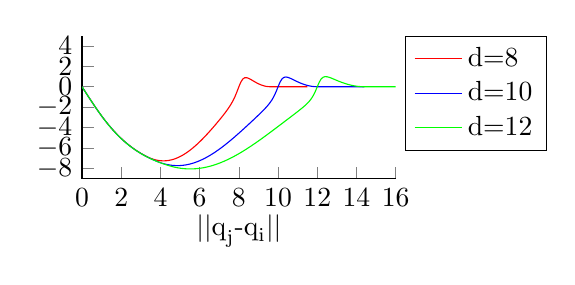
\begin{tikzpicture}

\begin{axis}[%
width=0.764\figW,
height=\figH,
at={(0\figW,0\figH)},
scale only axis,
every outer x axis line/.append style={black},
every x tick label/.append style={font=\color{black}},
xmin=0,
xmax=16,
xtick={ 0,  2,  4,  6,  8, 10, 12, 14, 16},
xlabel={$\text{$|$$|$q}_\text{j}\text{-q}_\text{i}\text{$|$$|$}$},
every outer y axis line/.append style={black},
every y tick label/.append style={font=\color{black}},
ymin=-9,
ymax=5,
ytick={-8, -6, -4, -2,  0,  2,  4},
axis background/.style={fill=white},
axis x line*=bottom,
axis y line*=left,
legend style={at={(1.03,1)},anchor=north west,legend cell align=left,align=left,draw=black},
xlabel shift={-4pt}
]
\addplot [color=red,solid]
  table[row sep=crcr]{%
0	-0\\
0.1	-0.299269979813303\\
0.2	-0.597643058396771\\
0.3	-0.89423566522595\\
0.4	-1.1881904311617\\
0.5	-1.47868816739967\\
0.6	-1.76495857491327\\
0.7	-2.04628938109857\\
0.8	-2.32203368864831\\
0.9	-2.59161541630041\\
1	-2.85453280457076\\
1.1	-3.11036004530868\\
1.2	-3.35874716678738\\
1.3	-3.59941836272638\\
1.4	-3.83216899265348\\
1.5	-4.05686150254159\\
1.6	-4.27342052024782\\
1.7	-4.48182737242136\\
1.8	-4.68211425123686\\
1.9	-4.87435823368657\\
2	-5.05867532619963\\
2.1	-5.23521467564571\\
2.2	-5.40415305642484\\
2.3	-5.565689713916\\
2.4	-5.7200416181107\\
2.5	-5.86743915840112\\
2.6	-6.00812229145813\\
2.7	-6.14233713887543\\
2.8	-6.27033301952284\\
2.9	-6.39235989297165\\
3	-6.50866618448829\\
3.1	-6.61949695848189\\
3.2	-6.72509240549032\\
3.3	-6.82548441921476\\
3.4	-6.91682840716877\\
3.5	-6.99739581724249\\
3.6	-7.06696004663902\\
3.7	-7.12532115863998\\
3.8	-7.17230728028945\\
3.9	-7.20777586691859\\
4	-7.23161482838137\\
4.1	-7.2437435124377\\
4.2	-7.24411354117508\\
4.3	-7.23270949669952\\
4.4	-7.20954945253926\\
4.5	-7.17468534727552\\
4.6	-7.12820319681719\\
4.7	-7.07022314143501\\
4.8	-7.00089932311255\\
4.9	-6.92041958788507\\
5	-6.8290050065197\\
5.1	-6.72690920500051\\
5.2	-6.61441749362011\\
5.3	-6.49184577976374\\
5.4	-6.35953924430114\\
5.5	-6.21787075429898\\
5.6	-6.06723897469503\\
5.7	-5.90806612740143\\
5.8	-5.74079532619918\\
5.9	-5.56588738698667\\
6	-5.38381697123676\\
6.1	-5.19506785936298\\
6.2	-5.00012705980656\\
6.3	-4.79947732257956\\
6.4	-4.59358741596941\\
6.5	-4.38289919784073\\
6.6	-4.16780999386659\\
6.7	-3.94864795625148\\
6.8	-3.72563669538053\\
6.9	-3.49884316013113\\
7	-3.2680987907865\\
7.1	-3.03287714411017\\
7.2	-2.79209938079827\\
7.3	-2.54381900913533\\
7.4	-2.28470616036701\\
7.5	-2.0092165859752\\
7.6	-1.70835597959428\\
7.7	-1.36834638738849\\
7.8	-0.971382891368651\\
7.9	-0.506207489026231\\
8	0\\
8.1	0.453554009433101\\
8.2	0.752629293324686\\
8.3	0.879755450057753\\
8.4	0.883854139704405\\
8.5	0.818498668673349\\
8.6	0.719579873848087\\
8.7	0.607837539496039\\
8.8	0.494933677043205\\
8.9	0.387571382825715\\
9	0.289767274919221\\
9.1	0.204045981388416\\
9.2	0.13206997843488\\
9.3	0.0749790876642189\\
9.4	0.0335787309657403\\
9.5	0.00844743638428441\\
9.6	0\\
9.7	0\\
9.8	0\\
9.9	0\\
10	0\\
10.1	0\\
10.2	0\\
10.3	0\\
10.4	0\\
10.5	0\\
10.6	0\\
10.7	0\\
10.8	0\\
10.9	0\\
11	0\\
11.1	0\\
11.2	0\\
11.3	0\\
11.4	0\\
11.5	0\\
};
\addlegendentry{d=8};

\addplot [color=blue,solid]
  table[row sep=crcr]{%
0	-0\\
0.1	-0.299528522991385\\
0.2	-0.598160545539665\\
0.3	-0.895012903830745\\
0.4	-1.18922864720793\\
0.5	-1.47998902282654\\
0.6	-1.76652419060389\\
0.7	-2.04812236513701\\
0.8	-2.32413716960111\\
0.9	-2.59399308128472\\
1	-2.85718894190541\\
1.1	-3.11329959160241\\
1.2	-3.36197575839647\\
1.3	-3.60294239160998\\
1.4	-3.83599566676511\\
1.5	-4.06099891101692\\
1.6	-4.27787770377923\\
1.7	-4.48661439934766\\
1.8	-4.68724230002036\\
1.9	-4.87983968260091\\
2	-5.06452385121079\\
2.1	-5.24144535763841\\
2.2	-5.41078249911034\\
2.3	-5.57273617395931\\
2.4	-5.72752514924123\\
2.5	-5.87538177152667\\
2.6	-6.01654813309575\\
2.7	-6.15127269055293\\
2.8	-6.27980732120194\\
2.9	-6.40240479401041\\
3	-6.51931662621179\\
3.1	-6.63079129308367\\
3.2	-6.73707275676515\\
3.3	-6.83839927972584\\
3.4	-6.93500248931646\\
3.5	-7.02710666141066\\
3.6	-7.11492819323542\\
3.7	-7.19867523788084\\
3.8	-7.27854747551985\\
3.9	-7.35470793877894\\
4	-7.42487372777091\\
4.1	-7.48746463863709\\
4.2	-7.54242999179877\\
4.3	-7.58972844876625\\
4.4	-7.62932834724765\\
4.5	-7.66120801141776\\
4.6	-7.6853560355767\\
4.7	-7.70177153974976\\
4.8	-7.71046439605667\\
4.9	-7.71145542491537\\
5	-7.70477656034584\\
5.1	-7.6904709838068\\
5.2	-7.6685932261351\\
5.3	-7.63920923726733\\
5.4	-7.60239642350644\\
5.5	-7.55824365215464\\
5.6	-7.50685122336834\\
5.7	-7.44833080909924\\
5.8	-7.38280535896901\\
5.9	-7.31040897287754\\
6	-7.23128674006506\\
6.1	-7.14559454422915\\
6.2	-7.05349883413071\\
6.3	-6.95517635889794\\
6.4	-6.85081386693846\\
6.5	-6.74060776697716\\
6.6	-6.62476374922418\\
6.7	-6.50349636400649\\
6.8	-6.37702855431856\\
6.9	-6.24559113759491\\
7	-6.10942223048574\\
7.1	-5.96876660839854\\
7.2	-5.82387498887069\\
7.3	-5.67500322420732\\
7.4	-5.52241138388909\\
7.5	-5.36636270050225\\
7.6	-5.20712234360245\\
7.7	-5.04495597286602\\
7.8	-4.880128003421\\
7.9	-4.71289948983074\\
8	-4.5435254969054\\
8.1	-4.37225176922386\\
8.2	-4.19931042727619\\
8.3	-4.0249142908797\\
8.4	-3.84924923439542\\
8.5	-3.67246367054386\\
8.6	-3.49465376754018\\
8.7	-3.31584220155749\\
8.8	-3.13594690974897\\
8.9	-2.95473403586483\\
9	-2.77174531633069\\
9.1	-2.58618319155126\\
9.2	-2.3967245068477\\
9.3	-2.20121164950207\\
9.4	-1.99613275241143\\
9.5	-1.77574995684846\\
9.6	-1.53071236815478\\
9.7	-1.24627361371349\\
9.8	-0.901959471552258\\
9.9	-0.480454389780927\\
10	-5.74441937126447e-15\\
10.1	0.450390555852559\\
10.2	0.764371901017294\\
10.3	0.917080471133783\\
10.4	0.951477073414525\\
10.5	0.916786535999093\\
10.6	0.8460466947438\\
10.7	0.758268247769631\\
10.8	0.664071376425615\\
10.9	0.569501792641379\\
11	0.478132914638606\\
11.1	0.392171963950856\\
11.2	0.313045091936783\\
11.3	0.241714388150343\\
11.4	0.1788548442931\\
11.5	0.124956233230472\\
11.6	0.0803835214364448\\
11.7	0.0454136907999905\\
11.8	0.0202587545144956\\
11.9	0.00508047863509588\\
12	0\\
12.1	0\\
12.2	0\\
12.3	0\\
12.4	0\\
12.5	0\\
12.6	0\\
12.7	0\\
12.8	0\\
12.9	0\\
13	0\\
13.1	0\\
13.2	0\\
13.3	0\\
13.4	0\\
13.5	0\\
13.6	0\\
13.7	0\\
13.8	0\\
13.9	0\\
14	0\\
14.1	0\\
14.2	0\\
14.3	0\\
14.4	0\\
};
\addlegendentry{d=10};

\addplot [color=green,solid]
  table[row sep=crcr]{%
0	-0\\
0.1	-0.299647681831648\\
0.2	-0.598398920018765\\
0.3	-0.895370609886431\\
0.4	-1.1897058645386\\
0.5	-1.48058600167814\\
0.6	-1.76724126055869\\
0.7	-2.0489599457032\\
0.8	-2.32509578237729\\
0.9	-2.59507336346152\\
1	-2.8583916608684\\
1.1	-3.1146256604141\\
1.2	-3.36342625195949\\
1.3	-3.60451856334581\\
1.4	-3.83769896568053\\
1.5	-4.06283099907186\\
1.6	-4.27984047351157\\
1.7	-4.4887099917525\\
1.8	-4.68947312272056\\
1.9	-4.88220842838242\\
2	-5.06703351702951\\
2.1	-5.244099264235\\
2.2	-5.41358431139603\\
2.3	-5.57568992235954\\
2.4	-5.73063525220569\\
2.5	-5.87865305943468\\
2.6	-6.01998587380583\\
2.7	-6.15488261686568\\
2.8	-6.2835956605265\\
2.9	-6.40637830054845\\
3	-6.52348261599892\\
3.1	-6.6351576822582\\
3.2	-6.74164810346857\\
3.3	-6.84319283007913\\
3.4	-6.94002422796288\\
3.5	-7.03236736716921\\
3.6	-7.12043950047189\\
3.7	-7.20444970427572\\
3.8	-7.28459865699687\\
3.9	-7.36107853261074\\
4	-7.43407298958207\\
4.1	-7.50375723779202\\
4.2	-7.5702981683183\\
4.3	-7.63385453298357\\
4.4	-7.69457716245383\\
4.5	-7.75250570813856\\
4.6	-7.80567461172651\\
4.7	-7.85329233163169\\
4.8	-7.89536532874662\\
4.9	-7.93190300104571\\
5	-7.96291785543279\\
5.1	-7.98842567032975\\
5.2	-8.00844564823009\\
5.3	-8.02300055762657\\
5.4	-8.03211686387744\\
5.5	-8.03582484870543\\
5.6	-8.03415871813146\\
5.7	-8.02715669873285\\
5.8	-8.01486112218825\\
5.9	-7.99731849812948\\
6	-7.97457957536646\\
6.1	-7.94669939158775\\
6.2	-7.91373731166654\\
6.3	-7.87575705472182\\
6.4	-7.83282671009819\\
6.5	-7.78501874243573\\
6.6	-7.73240998600424\\
6.7	-7.67508162847461\\
6.8	-7.61311918429404\\
6.9	-7.54661245782176\\
7	-7.47565549636714\\
7.1	-7.4003465332531\\
7.2	-7.32078792100329\\
7.3	-7.23708605472137\\
7.4	-7.14935128569397\\
7.5	-7.05769782520335\\
7.6	-6.96224363848119\\
7.7	-6.86311032866741\\
7.8	-6.76042301055554\\
7.9	-6.65431017380516\\
8	-6.54490353517655\\
8.1	-6.43233787918763\\
8.2	-6.31675088639972\\
8.3	-6.19828294829557\\
8.4	-6.07707696740672\\
8.5	-5.95327814095862\\
8.6	-5.8270337258052\\
8.7	-5.69849278178658\\
8.8	-5.56780588981841\\
8.9	-5.43512483994552\\
9	-5.30060228318162\\
9.1	-5.164391339089\\
9.2	-5.02664514856325\\
9.3	-4.88751635793743\\
9.4	-4.74715651597386\\
9.5	-4.60571535907731\\
9.6	-4.46333995143067\\
9.7	-4.3201736346642\\
9.8	-4.17635472454401\\
9.9	-4.03201486760083\\
10	-3.88727693491771\\
10.1	-3.74225227766663\\
10.2	-3.59703709022576\\
10.3	-3.45170750693114\\
10.4	-3.30631287319366\\
10.5	-3.16086633965829\\
10.6	-3.01533145875523\\
10.7	-2.86960269305542\\
10.8	-2.72347645418959\\
10.9	-2.57660707912217\\
11	-2.42843827584426\\
11.1	-2.27809364679319\\
11.2	-2.12419734681914\\
11.3	-1.96457315447497\\
11.4	-1.79573019950149\\
11.5	-1.61198175047604\\
11.6	-1.40399330646131\\
11.7	-1.15676505452971\\
11.8	-0.84864080896202\\
11.9	-0.458946231606757\\
12	0\\
12.1	0.443690089729577\\
12.2	0.764412500617351\\
12.3	0.932695233657069\\
12.4	0.987121613749085\\
12.5	0.973747875738061\\
12.6	0.923653976371904\\
12.7	0.854734464547454\\
12.8	0.776976174296139\\
12.9	0.696048440505536\\
13	0.615284164584707\\
13.1	0.536724337607174\\
13.2	0.461672138951829\\
13.3	0.390994175433836\\
13.4	0.325289325530241\\
13.5	0.264986392683904\\
13.6	0.210402310786876\\
13.7	0.161777822719098\\
13.8	0.119299919280333\\
13.9	0.0831162852462943\\
14	0.0533447992537326\\
14.1	0.0300799028836615\\
14.2	0.0133969468370054\\
14.3	0.00335520547982807\\
14.4	0\\
14.5	0\\
14.6	0\\
14.7	0\\
14.8	0\\
14.9	0\\
15	0\\
15.1	0\\
15.2	0\\
15.3	0\\
15.4	0\\
15.5	0\\
15.6	0\\
15.7	0\\
15.8	0\\
15.9	0\\
16	0\\
16.1	0\\
16.2	0\\
16.3	0\\
16.4	0\\
16.5	0\\
16.6	0\\
16.7	0\\
16.8	0\\
16.9	0\\
17	0\\
17.1	0\\
17.2	0\\
};
\addlegendentry{d=12};

\end{axis}
\end{tikzpicture}%
	    \caption{Influence of parameter d}
	\end{subfigure}

    \caption{Influence of the parameters on the action function}
    \label{fig:effects_actionCurve}
\end{figure} 

\subsection{Scenario}

We implemented this flocking strategy in a real-time swarm simulator. This simulator was developed in our lab and is capable of simulating the dynamics of many flying entities in real-time and faster than real-time. We used a challenging scenario, namely the circle scenario: each agent starts at a given position on the circle and has to travel through the center of circle, up to the opposite point of the circle. All agents start at the same time. If no collision avoidance strategy is used, a giant collision occurs in the center of the circle. 


\section{Design of Experiments}

We design the experiment to efficiently determine the influence of the  parameters $a$, $b$, and $d$ on the mean travel time and the mean total jerk experienced during the journey.

\subsection{Choosing a Model}
The complex nature of the problem does not allow to make assumptions on the model underlying the experiments. We therefore choose to investigate several models. We begin with a simple linear model of the form
\begin{subequations}\label{eq:model_lin}
\begin{align}
	y_a &= a_0 + \displaystyle\sum_{i=1}^{3} a_i x_i + \varepsilon_a \quad \text{and}\\ 
	y_b &= b_0 + \displaystyle\sum_{i=1}^{3} b_i x_i + \varepsilon_b,
\end{align}
\end{subequations}
where $y_a$ and $y_b$ are the responses (mean travel time and mean total jerk), $a_i$ and $b_i$ are the effects of the $i$th parameter on the travel time and the jerk respectively, $x_1$, $x_2$ and $x_3$ are the values taken by the parameters $a$, $b$ and $d$ respectively. Since the results of the analysis suggest that the influence of parameter $a$ on the travel time is negligible (cf. section~\ref{sec:results}), we adjust our model by omitting this parameter.
The nature of the algorithm suggest that interactions could play an important role. Hence, we will also investigate a linear model allowing for interactions between the parameters as described in eq.~\ref{eq:model_inter}.
\begin{subequations}\label{eq:model_inter}
\begin{align}
	y_a &= a_0 + \displaystyle\sum_{i=1}^{3} a_i x_i + \displaystyle\sum_{i,j=1, i \neq j}^{3} a_{ij} x_i x_j + \varepsilon_a \quad \text{and}\\ 
	y_b &= b_0 + \displaystyle\sum_{i=1}^{3} b_i x_i + \displaystyle\sum_{i,j=1, i \neq j}^{3} b_{ij} x_i x_j + \varepsilon_b
\end{align}
\end{subequations}
As for the linear model, we found that the influence of parameter $a$ and it's interactions is negligible and omit the parameter for the travel time. We also test a quadratic model with the following equations:
\begin{subequations}\label{eq:model_quadr}
\begin{align}
	y_a &= a_0 + \displaystyle\sum_{i=1}^{3} a_i x_i + \displaystyle\sum_{i,j=1}^{3} a_{ij} x_i x_j + \varepsilon_a \quad \text{and}\\ 
	y_b &= b_0 + \displaystyle\sum_{i=1}^{3} b_i x_i + \displaystyle\sum_{i,j=1}^{3} b_{ij} x_i x_j + \varepsilon_b,
\end{align}
\end{subequations}
which has additionally the quadratic factors $a_{ii}$.
Due to the limited number of experiments, we choose not to test higher order models.

\subsection{Choosing the Matrix of Experiments}
The matrix of experiments $E$ contains the levels, i.e., the values taken by the factors, normalized between $-1$ and $1$. Each row of $E$ corresponds to an experiment and each column to a factor. The choice of the matrix of experiments is crucial for an efficient estimation of the effects. While a high number of experiments $N$ yields a more accurate fit, experiments with flying platforms are costly in terms of time. The limits of the levels shown in tbl.~\ref{tbl:levels} were determined in preliminary experiment.
\begin{table}[h!]
	\centering
	\begin{tabular}{l r r r}
	 & $x_1$ (A) & $x_2$ (B) & $x_3$ (D) \\\hline
	min & 1 & 5 & 800\\
	max & 13 & 13 & 1400 \\
	\end{tabular}
	\caption{Maximal and minimal levels for each factor, found in perliminary experiments}\label{tbl:levels}
\end{table}
\begin{figure}[h]
    \centering
	\setlength{\abovecaptionskip}{1pt plus 3pt minus 0pt}
	\setlength{\figH}{0.25\textwidth}
	% This file was created by matlab2tikz.
%
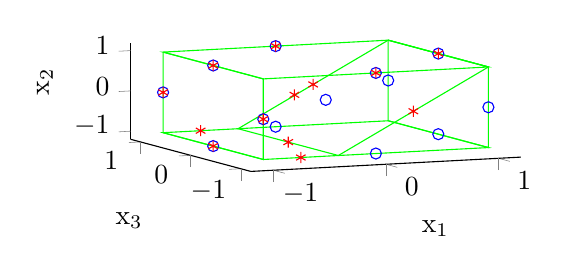
\begin{tikzpicture}

\begin{axis}[%
width=0.951\figW,
height=\figH,
at={(0\figW,0\figH)},
scale only axis,
every outer x axis line/.append style={black},
every x tick label/.append style={font=\color{black}},
xmin=-1.2,
xmax=1.2,
tick align=outside,
xlabel={$\text{x}_\text{1}$},
every outer y axis line/.append style={black},
every y tick label/.append style={font=\color{black}},
ymin=-1.2,
ymax=1.2,
ylabel={$\text{x}_\text{3}$},
every outer z axis line/.append style={black},
every z tick label/.append style={font=\color{black}},
zmin=-1.2,
zmax=1.2,
zlabel={$\text{x}_\text{2}$},
view={-24}{20},
axis background/.style={fill=white},
axis x line*=bottom,
axis y line*=left,
axis z line*=left,
xlabel shift={-4pt},
ylabel shift={-4pt}
]
\addplot3 [color=blue,only marks,mark=o,mark options={solid}]
 table[row sep=crcr] {%
-1	-1	0\\
-1	1	0\\
1	-1	0\\
1	1	0\\
-1	0	-1\\
-1	0	1\\
1	0	-1\\
1	0	1\\
0	-1	-1\\
0	-1	1\\
0	1	-1\\
0	1	1\\
0	0	0\\
};
 \addplot3 [color=red,only marks,mark=asterisk,mark options={solid}]
 table[row sep=crcr] {%
-1	-1	0\\
-1	1	0\\
0.333333333333333	-1	0\\
0.333333333333333	1	0\\
-1	0	-1\\
-1	0	1\\
-0.333333333333333	0	-1\\
1	0	1\\
-0.666666666666667	-1	-1\\
0	-1	1\\
-0.666666666666667	1	-1\\
-0.278333333333333	0	0.165\\
0	1	1\\
};
 \addplot3 [color=green,solid]
 table[row sep=crcr] {%
1	1	1\\
1	1	-1\\
1	-1	-1\\
1	-1	1\\
1	1	1\\
};
 \addplot3 [color=green,solid]
 table[row sep=crcr] {%
1	1	1\\
-1	1	1\\
-1	-1	1\\
1	-1	1\\
1	1	1\\
};
 \addplot3 [color=green,solid]
 table[row sep=crcr] {%
-1	1	1\\
-1	1	-1\\
-1	-1	-1\\
-1	-1	1\\
-1	1	1\\
};
 \addplot3 [color=green,solid]
 table[row sep=crcr] {%
1	1	-1\\
-1	1	-1\\
-1	-1	-1\\
1	-1	-1\\
1	1	-1\\
};
 \addplot3 [color=green,solid]
 table[row sep=crcr] {%
-0.333333333333333	-1	-1\\
-0.333333333333333	1	-1\\
1	1	1\\
1	-1	1\\
-0.333333333333333	-1	-1\\
};
 \end{axis}
\end{tikzpicture}%
    \caption{Chosen levels for the experiment: Original Box-Behnken design (in blue) and adjusted design (in red);}\label{fig:design}
\end{figure} 

The additional constraint $ x_1 \le x_2 $ is introduced by eq.~\ref{eq:phi}. To well cover the central values, we choose a Box-Behnken design~\cite{box_behnken} as shown in fig.~\ref{fig:design}. We adjust the values to fit our constraint by moving the points to the center of the sides of the truncated cube. The central point was moved to the center of gravity of the truncated cube. This results in the following matrix of experiments:
\begin{equation}
E = \begin{pmatrix}
		x_{11}  &  x_{12}  & x_{13} \\
		x_{21}  &  x_{22}  & x_{23} \\
		\vdots & \vdots & \vdots \\
		x_{N1} & x_{N2} & x_{N3}
		\end{pmatrix} = \begin{pmatrix}
		-1  &  0  & -1 \\
		-1  &  0  & -1 \\
		\nicefrac{1}{3} &	0	& -1 \\
		\nicefrac{1}{3} &	0	& 1  \\
		-1	&	-1	& 0 \\
		-1	&	1	& 0 \\
		-\nicefrac{1}{3} &	-1	& 0 \\
		1	  & -1  & 0 \\
		-\nicefrac{2}{3} &	-1	& -1 \\
		0	  &  1	& -1 \\
		-\nicefrac{2}{3} &	-1	& 1 \\
		-0.28 & 0.17 & 0 \\
		0 	& 1 	& 1 
		\end{pmatrix}
\end{equation}



\subsection{Estimating the effects}
We call $X$ the matrix of the matrix. Each row contains the levels of the factors and their products (if any) for one run of the experiment. For the quadratic model, $X$ takes the following form:
\begin{equation}
	\begin{pmatrix}
	1 & x_{11} & x_{12} & x_{13} & x_{11}^2 & x_{11} x_{12} & \cdots & x_{13}^2 \\
	1 & x_{21} & x_{22} & x_{23} & x_{21}^2 & x_{21} x_{22} & \cdots & x_{23}^2 \\
	 \vdots & \vdots & \vdots & \vdots & \vdots & \vdots & \ddots & \vdots\\
	1 & x_{N1} & x_{N2} & x_{N3} & x_{N1}^2 & x_{N1} x_{N2} & \cdots & x_{N3}^2 \\
	\end{pmatrix}
\end{equation}

The column vectors $Y_a$ and $Y_b$ contain the response in travel time and jerk where each element corresponds to the response to one run of the experiment.
Eq.~\ref{eq:model_lin}~to~\ref{eq:model_quadr} can then be formulated for all experiments as
\begin{equation}
 Y = X \hat{\alpha} + R = \hat{Y} + R,
\end{equation}
where $\hat{\alpha}$ is the column vector containing the estimated effects, $\hat{Y}$ are the estimated responses and $R$ is the residue column vector.

We estimate the effects (coefficients of the model) by minimizing the the residue in the sense of least square as expressed by eq. \ref{eq:least_square}.
\begin{equation}\label{eq:least_square}
	\hat\alpha =  \argmin_{\alpha}(\|Y - \hat{Y}\|^2) = \argmin_{\alpha}(\|R\|^2).
\end{equation}
The solution to eq. \ref{eq:least_square} can be computed as
\begin{equation}
	\hat\alpha = (X^T X)^{-1} X^{T} Y.
\end{equation}



\subsection{Analysis of Variance}
To evaluate our model, we use an F-test. We therefore define the sum of squares ($\text{SS}$) as
\begin{equation}
	\text{SS}_\text{eff} = \| \hat{Y} \|^2 = \| X \hat{\alpha} \|^2
\end{equation}
for the effects and as
\begin{equation}
	\text{SS}_\text{res} = \| R \|^2 = \| Y - \hat{Y} \| = \| Y - X \hat{\alpha} \|^2.
\end{equation}
The mean of squares ($\text{MS}$) as the distribution of the sum of squares ($\text{SS}$) over the degree's of freedom $\text{df}$:
\begin{equation}
	\text{MS}_\text{eff} = \frac{\text{SS}_\text{eff}}{\text{df}_\text{eff}} \quad \text{and} \quad 
	\text{MS}_\text{res} = \frac{\text{SS}_\text{res}}{\text{df}_\text{res}},
\end{equation}
where the degrees of freedom of the effects $\text{df}_\text{eff}$ is the number of effects including the constant and the degrees of freedom of the residue $\text{df}_\text{res}$ equals the number of experiment $N$ minus the degrees of freedom of the effects:
\begin{equation}
\text{df}_\text{res} = N - \text{df}_\text{eff}.
\end{equation}
We define Fisher's coefficient $F$ as follows:
\begin{equation}
F = \frac{\text{MS}_\text{eff}}{\text{MS}_\text{res}}.
\end{equation}

Using Fisher's coefficient, we can express the probability $p$ of this ratio occurring at random as the cumulative distribution function at $F$ for the degrees of freedom $\text{df}_\text{eff}$ and $\text{df}_\text{res}$:
\begin{equation}
	p = \int_{-\inf}^F f(t,\text{df}_\text{eff},\text{df}_\text{res}) \mathrm{d}t,
\end{equation}
where $f(x,\text{df}_1,\text{df}_2)$ is the probability density function of an F-distributed variable. Hence, the lower the p-value, the better is the model. We use the p-value as a metric to measure the performance of our model.


\section{Results}\label{sec:results}


\subsection{Linear Model}
First, we will discuss the results for the linear model.
Fig. \ref{fig:effects_lin} shows the half effects for both the travel time and the jerk in blue. It can be seen that the influence of parameter A (coefficients $a_1$ and $b_1$) on both the travel time and the jerk is negligible compared to the other effects.
\begin{figure}[h]
    \centering
    \begin{subfigure}[b]{0.5\textwidth}
		\setlength{\abovecaptionskip}{1pt plus 3pt minus 0pt}	
	    % This file was created by matlab2tikz.
%
\definecolor{mycolor1}{rgb}{0.20000,0.20000,0.50000}%
\definecolor{mycolor2}{rgb}{0.00000,0.70000,0.70000}%
%
\begin{tikzpicture}

\begin{axis}[%
width=0.951\figW,
height=\figH,
at={(0\figW,0\figH)},
scale only axis,
separate axis lines,
every outer x axis line/.append style={black},
every x tick label/.append style={font=\color{black}},
xmin=0.5,
xmax=4.5,
xtick={1,2,3,4},
xticklabels={{$a_0$},{$a_1$},{$a_2$},{$a_3$},{$a_{12}$},{$a_{13}$},{$a_{23}$},{$a_{11}$},{$a_{22}$},{$a_{33}$}},
xlabel={coefficients},
every outer y axis line/.append style={black},
every y tick label/.append style={font=\color{black}},
ymin=0,
ymax=1,
ylabel={$\text{a}_\text{i}\text{/a}_\text{0}$},
axis background/.style={fill=white},
xlabel shift={-4pt},
ylabel shift={-4pt}
]
\addplot[ybar,bar width=0.5,draw=black,fill=mycolor1,area legend] plot table[row sep=crcr] {%
1	1\\
2	0.00339552585792994\\
3	0.27192029312426\\
4	0.201983314513812\\
};
\addplot [color=black,solid,forget plot]
  table[row sep=crcr]{%
0.5	0\\
4.5	0\\
};
\addplot[ybar,bar width=0.25,draw=black,fill=mycolor2,area legend] plot table[row sep=crcr] {%
1	0.998868158047356\\
3	0.273052135076903\\
4	0.201983314513812\\
};
\end{axis}
\end{tikzpicture}%
	    \caption{travel time}
	\end{subfigure}
	%\par\medskip
    \begin{subfigure}[b]{0.5\textwidth}
	    \setlength{\abovecaptionskip}{1pt plus 3pt minus 0pt}
	    % This file was created by matlab2tikz.
%
\definecolor{mycolor1}{rgb}{0.20000,0.20000,0.50000}%
\definecolor{mycolor2}{rgb}{0.00000,0.70000,0.70000}%
%
\begin{tikzpicture}

\begin{axis}[%
width=0.951\figW,
height=\figH,
at={(0\figW,0\figH)},
scale only axis,
separate axis lines,
every outer x axis line/.append style={black},
every x tick label/.append style={font=\color{black}},
xmin=0.5,
xmax=4.5,
xtick={1,2,3,4},
xticklabels={{$b_0$},{$b_1$},{$b_2$},{$b_3$},{$b_{12}$},{$b_{13}$},{$b_{23}$},{$b_{11}$},{$b_{22}$},{$b_{33}$}},
xlabel={coefficients},
every outer y axis line/.append style={black},
every y tick label/.append style={font=\color{black}},
ymin=0,
ymax=1,
ylabel={bi/bo},
axis background/.style={fill=white},
xlabel shift={-4pt},
ylabel shift={-5pt}
]
\addplot[ybar,bar width=0.5,draw=black,fill=mycolor1,area legend] plot table[row sep=crcr] {%
1	1\\
2	0.0572355129983193\\
3	0.822964208269701\\
4	0.479348852445352\\
};
\addplot [color=black,solid,forget plot]
  table[row sep=crcr]{%
0.5	0\\
4.5	0\\
};
\addplot[ybar,bar width=0.25,draw=black,fill=mycolor2,area legend] plot table[row sep=crcr] {%
1	0.980921495667227\\
3	0.842042712602474\\
4	0.479348852445352\\
};
\end{axis}
\end{tikzpicture}%
   	    \caption{jerk}
	\end{subfigure}
	
    \caption{Relative half effects on the mean travel time (a) and the mean experienced jerk (b) using a linear model without interactions; In blue results for using all parameters and in turquoise if omitting parameter A (coefficients $a1$ and $b1$)}\label{fig:effects_lin}
\end{figure} 

The ANOVA table of the experiment is shown in tbl. \ref{tbl:anova_lin}. The p-value for the travel time model (2.35e-7) is significantly lower than the p-value for jerk model (4.72e-2). This suggest that the travel time model fits much better the experimental data.

\begin{table}[h!]
	\centering
	\begin{tabular}{l l r r r r r}
Resp & Src & $\text{SS}$ & $\text{df}$ & $\text{MS}$ & $F$  &  $p$\\\hline
      Time	 & $    \alpha          	$ & 34.42	 & 4  	 & 8.606	 & 95.04	 & 2.3e-07\\
          	 & $         R          	$ & 0.815	 & 9  	 & 0.09055 \\ 
\arrayrulecolor{gray}\hline
      Time	 & $    \alpha        ^1	$ & 34.42	 & 3  	 & 11.47	 & 140.8	 & 1.8e-08\\
          	 & $         R        ^1	$ & 0.8151	 & 10 	 & 0.08151 \\ 
\arrayrulecolor{gray}\hline
      Jerk	 & $    \alpha          	$ & 2406	 & 4  	 & 601.5	 & 3.718	 & 0.047\\
          	 & $         R          	$ & 1456	 & 9  	 & 161.8 \\ 
\arrayrulecolor{gray}\hline
      Jerk	 & $    \alpha        ^1	$ & 2404	 & 3  	 & 801.5	 & 5.498	 & 0.017\\
          	 & $         R        ^1	$ & 1458	 & 10 	 & 145.8 \\ 

	\end{tabular}
	\caption{ANOVA table of the \textbf{linear model} for both responses; The $^1$ indicates the model without parameter A; It shows the sums of squares (SS), the degrees of freedom (df), the mean square of the error (MS), the Fisher coefficient (F) and the p-value (p), signifying the probability that this result occurs at random;}\label{tbl:anova_lin}
\end{table}

%Fig. \ref{fig:interpol_lin1} shows the experimental results for the travel time as well as the planes representing the interpolation using the effects that we have found. The colors correspond to different values of parameter C, i.e., the dots should be close to the plane of the same color.
%Fig. \ref{fig:interpol_lin2} shows the results in terms of jerk. Note that here the colors correspond to the value of the parameter A. It can be seen that the points for measurements with the same values for parameter B and C are close by, encouraging the assumption that the influence of parameter A is negligible.

%We therefore adjust both our models by omitting parameter A.
We adjust both out models by omitting parameter A. We expect the residue to increase slightly since we remove a degree of freedom. The removal of a degree of freedom should however increase F-factor and therefore reduce the p-value, since the residue gains a degree of freedom. The resulting estimation of the half effects is shown in fig. \ref{fig:effects_lin} in turquoise. It can be seen that the values of the half effects are similar to the previous results.

When comparing the values in the ANOVA table, it can be seen that the $p$ value decreases by a factor of approximately 13 for the travel time, suggesting that omitting parameter A is improving our model. For the model of the jerk, the p-value decreases by a factor of approximately 2.7.


\subsection{Linear Model with interactions}

\begin{figure}[h]
    \centering
    \begin{subfigure}[b]{0.5\textwidth}
	    \setlength{\abovecaptionskip}{1pt plus 3pt minus 0pt}
	    % This file was created by matlab2tikz.
%
\definecolor{mycolor1}{rgb}{0.20000,0.20000,0.50000}%
\definecolor{mycolor2}{rgb}{0.00000,0.70000,0.70000}%
%
\begin{tikzpicture}

\begin{axis}[%
width=0.951\figW,
height=\figH,
at={(0\figW,0\figH)},
scale only axis,
separate axis lines,
every outer x axis line/.append style={black},
every x tick label/.append style={font=\color{black}},
xmin=0,
xmax=8,
xtick={1,2,3,4,5,6,7},
xticklabels={{$a_0$},{$a_1$},{$a_2$},{$a_3$},{$a_{12}$},{$a_{13}$},{$a_{23}$},{$a_{11}$},{$a_{22}$},{$a_{33}$}},
xlabel={coefficients},
every outer y axis line/.append style={black},
every y tick label/.append style={font=\color{black}},
ymin=-0.2,
ymax=1.2,
ylabel={ai/ao},
axis background/.style={fill=white},
xlabel shift={-4pt}
]
\addplot[ybar,bar width=0.5,draw=black,fill=mycolor1,area legend] plot table[row sep=crcr] {%
1	1\\
2	-0.000158480987423072\\
3	0.276585231712786\\
4	0.202308189537893\\
5	0.00801820250102874\\
6	-0.000745454946096567\\
7	0.116456628245764\\
};
\addplot [color=black,solid,forget plot]
  table[row sep=crcr]{%
0	0\\
8	0\\
};
\addplot[ybar,bar width=0.25,draw=black,fill=mycolor2,area legend] plot table[row sep=crcr] {%
1	1\\
3	0.273361537132869\\
4	0.202212186750112\\
7	0.116010508284771\\
};
\end{axis}
\end{tikzpicture}%
	    \caption{travel time}
	\end{subfigure}
    \begin{subfigure}[b]{0.5\textwidth}
		\setlength{\abovecaptionskip}{1pt plus 3pt minus 0pt}	
	    % This file was created by matlab2tikz.
%
\definecolor{mycolor1}{rgb}{0.20000,0.20000,0.50000}%
\definecolor{mycolor2}{rgb}{0.00000,0.70000,0.70000}%
%
\begin{tikzpicture}

\begin{axis}[%
width=0.951\figW,
height=\figH,
at={(0\figW,0\figH)},
scale only axis,
separate axis lines,
every outer x axis line/.append style={black},
every x tick label/.append style={font=\color{black}},
xmin=0,
xmax=8,
xtick={1,2,3,4,5,6,7},
xticklabels={{$b_0$},{$b_1$},{$b_2$},{$b_3$},{$b_{12}$},{$b_{13}$},{$b_{23}$},{$b_{11}$},{$b_{22}$},{$b_{33}$}},
xlabel={coefficients},
every outer y axis line/.append style={black},
every y tick label/.append style={font=\color{black}},
ymin=-0.2,
ymax=1.2,
ylabel={bi/bo},
axis background/.style={fill=white},
xlabel shift={-4pt}
]
\addplot[ybar,bar width=0.5,draw=black,fill=mycolor1,area legend] plot table[row sep=crcr] {%
1	1\\
2	0.0492031949956049\\
3	0.837675184978511\\
4	0.479930485262015\\
5	0.0189360359982001\\
6	-0.0078955424930121\\
7	0.0133129711999519\\
};
\addplot [color=black,solid,forget plot]
  table[row sep=crcr]{%
0	0\\
8	0\\
};
\addplot[ybar,bar width=0.25,draw=black,fill=mycolor2,area legend] plot table[row sep=crcr] {%
1	1\\
3	0.858420083892354\\
4	0.488671982990134\\
};
\end{axis}
\end{tikzpicture}%
   	    \caption{jerk}
	\end{subfigure}
	
    \caption{Relative half effects on the mean travel time (a) and the mean experienced jerk (b) using a \textbf{linear model with interactions}; In blue results for using all parameters and in turquoise if omitting coefficients $a_{1}$, $a_{12}$ and $a_{13}$ and $b_{1}$, $b_{12}$, $b_{13}$, and $b_{23}$)}\label{fig:effects_lin_interactions}
\end{figure} 
Fig. \ref{fig:effects_lin_interactions} shows the effects for this model. For both response variables we can again see that the influences of parameter A is negligible as it was the case for the purely linear model. Furthermore, the interactions appear to be negligible in the case of the jerk model. Considering the ANOVA table for this model (tbl. \ref{tbl:anova_lin_interactions}), it can be seen that the p value is significantly higher than for the linear model. This suggests that the addition of the interactions does not improve the model. This is due to the fact that the number of degrees of freedom of the models increase significantly were as whereas the residues remain approximately the same as for the linear models. While removing parameter A from the travel time model reduces it's p-value, it still remains inferior to the linear model.

\begin{table}[h!]
	\centering
	\begin{tabular}{l l r r r r r}
Resp & Src & $\text{SS}$ & $\text{df}$ & $\text{MS}$ & $F$  &  $p$\\\hline
      Time	 & $    \alpha          	$ & 34.56	 & 7  	 & 4.936	 & 43.4	 & 0.0001\\
          	 & $         R          	$ & 0.6825	 & 6  	 & 0.1137 \\ 
\arrayrulecolor{gray}\hline
      Time	 & $    \alpha        ^1	$ & 33.62	 & 4  	 & 8.405	 & 46.75	 & 5e-06\\
          	 & $         R        ^1	$ & 1.618	 & 9  	 & 0.1798 \\ 
\arrayrulecolor{gray}\hline
      Jerk	 & $    \alpha          	$ & 2406	 & 7  	 & 343.7	 & 1.416	 & 0.34\\
          	 & $         R          	$ & 1456	 & 6  	 & 242.7 \\ 
\arrayrulecolor{gray}\hline

	\end{tabular}

	\caption{ANOVA table of the \textbf{linear model with interactions}; The $^1$ indicates the model without the coefficients $a_{1}$, $a_{12}$, and $a_{13}$;)}\label{tbl:anova_lin_interactions}
\end{table}



\subsection{Quadratic Model}

\begin{figure}[h]
    \centering
    \begin{subfigure}[b]{0.5\textwidth}
	    \setlength{\abovecaptionskip}{1pt plus 3pt minus 0pt}
	    % This file was created by matlab2tikz.
%
\definecolor{mycolor1}{rgb}{0.20000,0.20000,0.50000}%
\definecolor{mycolor2}{rgb}{0.00000,0.70000,0.70000}%
%
\begin{tikzpicture}

\begin{axis}[%
width=0.951\figW,
height=\figH,
at={(0\figW,0\figH)},
scale only axis,
separate axis lines,
every outer x axis line/.append style={black},
every x tick label/.append style={font=\color{black}},
xmin=0,
xmax=12,
xtick={1,2,3,4,5,6,7,8,9,10},
xticklabels={{$a_0$},{$a_1$},{$a_2$},{$a_3$},{$a_{12}$},{$a_{13}$},{$a_{23}$},{$a_{11}$},{$a_{22}$},{$a_{33}$}},
xlabel={coefficients},
every outer y axis line/.append style={black},
every y tick label/.append style={font=\color{black}},
ymin=-0.4,
ymax=1,
ylabel={$\text{a}_\text{i}\text{/a}_\text{0}$},
axis background/.style={fill=white},
xlabel shift={-4pt},
ylabel shift={-4pt}
]
\addplot[ybar,bar width=0.5,draw=black,fill=mycolor1,area legend] plot table[row sep=crcr] {%
1	1\\
2	0.239284478024578\\
3	0.120506889726704\\
4	0.204107368761907\\
5	-0.231907710805712\\
6	-0.000752084470361102\\
7	0.117492307258645\\
8	0.358503129231724\\
9	0.0384436095354865\\
10	-0.0964862476571698\\
};
\addplot [color=black,solid,forget plot]
  table[row sep=crcr]{%
0	0\\
12	0\\
};
\addplot[ybar,bar width=0.25,draw=black,fill=mycolor2,area legend] plot table[row sep=crcr] {%
1	1\\
2	0.239284478024579\\
3	0.120506889726704\\
4	0.204358063585361\\
5	-0.231907710805709\\
7	0.117241612435192\\
8	0.358503129231725\\
9	0.0384436095354871\\
10	-0.0964862476571693\\
};
\end{axis}
\end{tikzpicture}%
	    \caption{travel time}
	\end{subfigure}
    \begin{subfigure}[b]{0.5\textwidth}
		\setlength{\abovecaptionskip}{1pt plus 3pt minus 0pt}	
	    % This file was created by matlab2tikz.
%
\definecolor{mycolor1}{rgb}{0.20000,0.20000,0.50000}%
\definecolor{mycolor2}{rgb}{0.00000,0.70000,0.70000}%
%
\begin{tikzpicture}

\begin{axis}[%
width=0.951\figW,
height=\figH,
at={(0\figW,0\figH)},
scale only axis,
separate axis lines,
every outer x axis line/.append style={black},
every x tick label/.append style={font=\color{black}},
xmin=0,
xmax=12,
xtick={0,1,2,3,4,5,6,7,8,9,10},
xticklabels={{$b_0$},{$b_1$},{$b_2$},{$b_3$},{$b_{12}$},{$b_{13}$},{$b_{23}$},{$b_{11}$},{$b_{22}$},{$b_{33}$}},
xlabel={coefficients},
every outer y axis line/.append style={black},
every y tick label/.append style={font=\color{black}},
ymin=-2,
ymax=3,
ylabel={bi/bo},
axis background/.style={fill=white},
xlabel shift={-4pt},
ylabel shift={-5pt}
]
\addplot[ybar,bar width=0.5,draw=black,fill=mycolor1,area legend] plot table[row sep=crcr] {%
1	1\\
2	1.86406685964224\\
3	-0.227113190318953\\
4	0.544838197826409\\
5	-1.73747866012659\\
6	-0.0089633671434854\\
7	0.0151134705109152\\
8	2.77139409919224\\
9	0.181327519247342\\
10	-0.576998447029369\\
};
\addplot [color=black,solid,forget plot]
  table[row sep=crcr]{%
0	0\\
12	0\\
};
\addplot[ybar,bar width=0.25,draw=black,fill=mycolor2,area legend] plot table[row sep=crcr] {%
1	1\\
2	1.86406685964224\\
3	-0.227113190318953\\
4	0.547825986874237\\
5	-1.73747866012659\\
8	2.77139409919224\\
9	0.181327519247342\\
10	-0.576998447029369\\
};
\end{axis}
\end{tikzpicture}%
   	    \caption{jerk}
	\end{subfigure}
	
    \caption{Relative half effects on the mean travel time (a) and the mean experienced jerk (b) using a \textbf{quadratic model}; In blue results for using all parameters and in turquoise if omitting coefficients $a_{13}$ and $b_{13}$ and $b_{23}$}\label{fig:effects_quadr}
\end{figure} 


Fig. \ref{fig:effects_quadr} shows the effects for the quadratic model. Interestingly, in this model parameter A has the largest influence on both the mean travel time and the mean experienced jerk.
%Fig. \ref{fig:interpol_quadr} shows the experimental values as well as the quadratic interpolation for the mean arrival time.
Considering the ANOVA table (tbl.~\ref{tbl:anova_quadratic}), it can be seen that the residue is smaller than for the other models. However, this is mainly due to the fact of introducing additional degrees of freedom. Furthermore, the ANOVA table shows that the p-value is higher than for the linear model, suggesting that the quality of model decreases by introducing quadratic terms.
We adjust our models by removing the coefficients $a_{13}$ from the travel time model and the coefficients $b_{13}$ and $b_{23}$ from the jerk model.

\begin{table}[h!]
	\centering
	\begin{tabular}{@{} l @{\hspace{8pt}} l @{\hspace{8pt}} r @{\hspace{8pt}} r @{\hspace{8pt}} r @{\hspace{8pt}} r r @{}}
Resp & Src & $\text{SS}$ & $\text{df}$ & $\text{MS}$ & $F$  &  $p$\\\hline
      Time	 & $    \alpha          	$ & 35.1	 & 10 	 & 3.51	 & 81.7	 & 1.98e-03\\
          	 & $         R          	$ & 0.129	 & 3  	 & 0.043 \\ 
\arrayrulecolor{gray}\hline
      Time	 & $    \alpha        ^1	$ & 35.1	 & 9  	 & 3.9	 & 121	 & 1.64e-04\\
          	 & $         R        ^1	$ & 0.129	 & 4  	 & 0.0322 \\ 
\arrayrulecolor{gray}\hline
      Jerk	 & $    \alpha          	$ & 3.54e+03	 & 10 	 & 354	 & 3.3	 & 1.78e-01\\
          	 & $         R          	$ & 322	 & 3  	 & 107 \\ 
\arrayrulecolor{gray}\hline
      Jerk	 & $    \alpha        ^2	$ & 3.54e+03	 & 9  	 & 393	 & 4.88	 & 7.06e-02\\
          	 & $         R        ^2	$ & 322	 & 4  	 & 80.6 \\ 

	\end{tabular}

	\caption{ANOVA table of the \textbf{quadratic} model; The $^1$ indicates the model without the coefficient $a_{13}$ and $^2$ without coefficients $b_{13}$, $b_{23}$;}\label{tbl:anova_quadratic}
\end{table}


\section{Conclusion}

In this work, we investigated the influence of three parameters on the performance of a collision avoiding algorithm design to allow collision free navigation of autonomous aerial vehicles. We measured the performance of the algorithm in terms of the mean travel time as well as the mean jerk that would be experienced by a passenger in a vehicles during the travel.

Due to technical issues on the platform, we decided to perform the experiment in simulation.
We fitted three different models on the experimental data: A purely linear model, a linear model allowing for interactions and a quadratic model allowing for linear interactions.

By comparing the p-value of the models, the linear model has been found to be the best model for modelling both the mean travel time and the mean experienced jerk. The p-values for both responses lay below the confidence level. We found that the influence of parameter $a$ is negligible for both responses. Therefore, we adjusted the model by removing parameter $a$. This improves the confidence of the fit and reduces the model's complexity.

\begin{figure}[h]
	\centering
	%\setlength{\figW}{0.43\textwidth}
    %\begin{subfigure}[b]{0.5\textwidth}
		\setlength{\figH}{0.23\textwidth}
		% This file was created by matlab2tikz.
%
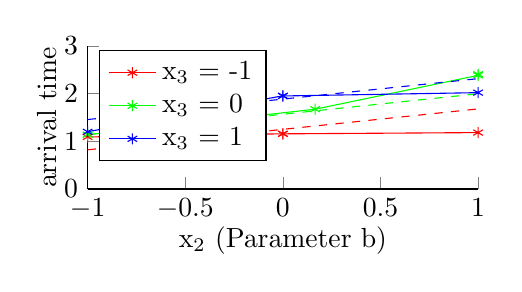
\begin{tikzpicture}

\begin{axis}[%
width=0.951\figW,
height=\figH,
at={(0\figW,0\figH)},
scale only axis,
every outer x axis line/.append style={black},
every x tick label/.append style={font=\color{black}},
xmin=-1,
xmax=1,
xlabel={$\text{x}_\text{2}\text{ (Parameter b)}$},
every outer y axis line/.append style={black},
every y tick label/.append style={font=\color{black}},
ymin=0,
ymax=3,
ylabel={arrival time},
axis background/.style={fill=white},
axis x line*=bottom,
axis y line*=left,
legend style={at={(0.03,0.97)},anchor=north west,legend cell align=left,align=left,draw=black},
xlabel shift={-4pt},
ylabel shift={-4pt}
]
\addplot [color=red,solid,mark=asterisk,mark options={solid}]
  table[row sep=crcr]{%
-1	1.09053213545266\\
0	1.15704906703525\\
0	1.15618521078093\\
1	1.18227366966137\\
};
\addlegendentry{$\text{x}_\text{3}\text{ = -1}$};

\addplot [color=green,solid,mark=asterisk,mark options={solid}]
  table[row sep=crcr]{%
-1	1.13873531444368\\
-1	1.13769868693849\\
0.165	1.6720801658604\\
1	2.38113337940567\\
1	2.40601243953006\\
};
\addlegendentry{$\text{x}_\text{3}\text{ = 0}$};

\addplot [color=blue,solid,mark=asterisk,mark options={solid}]
  table[row sep=crcr]{%
-1	1.19989633724948\\
0	1.95317899101589\\
0	1.94920525224603\\
1	2.01883206634416\\
};
\addlegendentry{$\text{x}_\text{3}\text{ = 1}$};

\addplot [color=red,dashed,forget plot]
  table[row sep=crcr]{%
-1	0.821821551505145\\
-0.9	0.864659680103842\\
-0.8	0.907497808702539\\
-0.7	0.950335937301236\\
-0.6	0.993174065899933\\
-0.5	1.03601219449863\\
-0.4	1.07885032309733\\
-0.3	1.12168845169602\\
-0.2	1.16452658029472\\
-0.1	1.20736470889342\\
0	1.25020283749211\\
0.1	1.29304096609081\\
0.2	1.33587909468951\\
0.3	1.37871722328821\\
0.4	1.4215553518869\\
0.5	1.4643934804856\\
0.6	1.5072316090843\\
0.7	1.55006973768299\\
0.8	1.59290786628169\\
0.9	1.63574599488039\\
1	1.67858412347908\\
};
\addplot [color=green,dashed,forget plot]
  table[row sep=crcr]{%
-1	1.13870562199582\\
-0.9	1.18154375059451\\
-0.8	1.22438187919321\\
-0.7	1.26722000779191\\
-0.6	1.3100581363906\\
-0.5	1.3528962649893\\
-0.4	1.395734393588\\
-0.3	1.43857252218669\\
-0.2	1.48141065078539\\
-0.1	1.52424877938409\\
0	1.56708690798279\\
0.1	1.60992503658148\\
0.2	1.65276316518018\\
0.3	1.69560129377888\\
0.4	1.73843942237757\\
0.5	1.78127755097627\\
0.6	1.82411567957497\\
0.7	1.86695380817366\\
0.8	1.90979193677236\\
0.9	1.95263006537106\\
1	1.99546819396975\\
};
\addplot [color=blue,dashed,forget plot]
  table[row sep=crcr]{%
-1	1.45558969248649\\
-0.9	1.49842782108518\\
-0.8	1.54126594968388\\
-0.7	1.58410407828258\\
-0.6	1.62694220688127\\
-0.5	1.66978033547997\\
-0.4	1.71261846407867\\
-0.3	1.75545659267736\\
-0.2	1.79829472127606\\
-0.1	1.84113284987476\\
0	1.88397097847346\\
0.1	1.92680910707215\\
0.2	1.96964723567085\\
0.3	2.01248536426955\\
0.4	2.05532349286824\\
0.5	2.09816162146694\\
0.6	2.14099975006564\\
0.7	2.18383787866433\\
0.8	2.22667600726303\\
0.9	2.26951413586173\\
1	2.31235226446042\\
};
\end{axis}
\end{tikzpicture}%
		\caption{travel time}\label{fig:concl_time}
\end{figure}	
\begin{figure}
    %\begin{subfigure}[b]{0.5\textwidth}
    		\centering
		\setlength{\figH}{0.23\textwidth}		
		% This file was created by matlab2tikz.
%
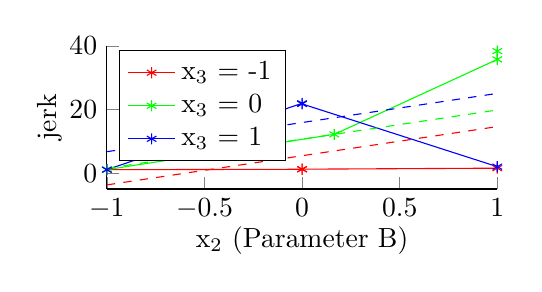
\begin{tikzpicture}

\begin{axis}[%
width=0.951\figW,
height=\figH,
at={(0\figW,0\figH)},
scale only axis,
every outer x axis line/.append style={black},
every x tick label/.append style={font=\color{black}},
xmin=-1,
xmax=1,
xlabel={$\text{x}_\text{2}\text{ (Parameter B)}$},
every outer y axis line/.append style={black},
every y tick label/.append style={font=\color{black}},
ymin=-5,
ymax=40,
ylabel={jerk},
axis background/.style={fill=white},
axis x line*=bottom,
axis y line*=left,
legend style={at={(0.03,0.97)},anchor=north west,legend cell align=left,align=left,draw=black},
xlabel shift={-4pt},
ylabel shift={-4pt}
]
\addplot [color=red,solid,mark=asterisk,mark options={solid}]
  table[row sep=crcr]{%
-1	1.06763197356231\\
0	1.20482048539146\\
0	1.23116266631009\\
1	1.54848024654804\\
};
\addlegendentry{$\text{x}_\text{3}\text{ = -1}$};

\addplot [color=green,solid,mark=asterisk,mark options={solid}]
  table[row sep=crcr]{%
-1	1.09509641925902\\
-1	1.09375766084999\\
0.165	12.1805684231304\\
1	35.7252695823265\\
1	38.333221902788\\
};
\addlegendentry{$\text{x}_\text{3}\text{ = 0}$};

\addplot [color=blue,solid,mark=asterisk,mark options={solid}]
  table[row sep=crcr]{%
-1	1.07879572234055\\
0	21.9381273937669\\
0	21.7369156661796\\
1	2.02139784843536\\
};
\addlegendentry{$\text{x}_\text{3}\text{ = 1}$};

\addplot [color=red,dashed,forget plot]
  table[row sep=crcr]{%
-1	-3.70436914752427\\
-0.9	-2.78821312501782\\
-0.8	-1.87205710251137\\
-0.7	-0.955901080004915\\
-0.6	-0.0397450574984664\\
-0.5	0.876410965007984\\
-0.4	1.79256698751443\\
-0.3	2.70872301002088\\
-0.2	3.62487903252733\\
-0.1	4.54103505503378\\
0	5.45719107754023\\
0.1	6.37334710004668\\
0.2	7.28950312255313\\
0.3	8.20565914505958\\
0.4	9.12181516756603\\
0.5	10.0379711900725\\
0.6	10.9541272125789\\
0.7	11.8702832350854\\
0.8	12.7864392575918\\
0.9	13.7025952800983\\
1	14.6187513026047\\
};
\addplot [color=green,dashed,forget plot]
  table[row sep=crcr]{%
-1	1.51102350983954\\
-0.9	2.42717953234599\\
-0.8	3.34333555485244\\
-0.7	4.25949157735889\\
-0.6	5.17564759986534\\
-0.5	6.09180362237179\\
-0.4	7.00795964487824\\
-0.3	7.92411566738469\\
-0.2	8.84027168989114\\
-0.1	9.75642771239759\\
0	10.672583734904\\
0.1	11.5887397574105\\
0.2	12.5048957799169\\
0.3	13.4210518024234\\
0.4	14.3372078249298\\
0.5	15.2533638474363\\
0.6	16.1695198699427\\
0.7	17.0856758924492\\
0.8	18.0018319149556\\
0.9	18.9179879374621\\
1	19.8341439599685\\
};
\addplot [color=blue,dashed,forget plot]
  table[row sep=crcr]{%
-1	6.72641616720335\\
-0.9	7.6425721897098\\
-0.8	8.55872821221625\\
-0.7	9.4748842347227\\
-0.6	10.3910402572292\\
-0.5	11.3071962797356\\
-0.4	12.2233523022421\\
-0.3	13.1395083247485\\
-0.2	14.055664347255\\
-0.1	14.9718203697614\\
0	15.8879763922678\\
0.1	16.8041324147743\\
0.2	17.7202884372808\\
0.3	18.6364444597872\\
0.4	19.5526004822936\\
0.5	20.4687565048001\\
0.6	21.3849125273065\\
0.7	22.301068549813\\
0.8	23.2172245723194\\
0.9	24.1333805948259\\
1	25.0495366173323\\
};
\end{axis}
\end{tikzpicture}%
		\caption{jerk}\label{fig:concl_jerk}
	%\end{subfigure}
	%\caption{hello}\label{fig:concl_fit}
\end{figure}

Fig. \ref{fig:concl_time} shows the experimental values for the mean travel time and the linearly interpolated data. The linear fit for the jerk can be seen in fig. \ref{fig:concl_jerk}. It can be seen that the fit for the travel time is more accurate than for the jerk. This is encouraged by a comparison of the p-value. While the travel time model has a p-value of 1.78e-8, the jerk model as a p-value of 0.0172. While the model for the travel time has an acceptable p-value, the reliability of the model for the jerk is less convincing.

We conclude that parameter $a$ is negligible for both the travel time and the jerk. Furthermore, both responses are assumed to depend linearly on parameters $b$ and $c$.

\end{document}